% !TeX root = main.tex

\section{奇异同调论}

\subsection{相对同调}

对子复形 $ K_0\subset K $, 它们的链复形 $ \CC(K_0) $ 与 $ \CC(K) $ 满足
\[
	C_p(K_0)\leqslant C_p(K),\quad S_p^+(K_0)\subset S_p^+(K).
\]
于是 $ C_p(K)/C_p(K_0) $ 仍是自由 Abel 群.

\begin{Definition}[相对链群, 相对链复形, 相对同调群]
	设 $ K_0 $ 是 $ K $ 的子复形, 称
	\[
		C_p(K,K_0)=C_p(K)/C_p(K_0)
	\]
	是 $ K $ 模 $ K_0 $ 的\emph{相对链群}. 它是自由 Abel 群, 其中的元素为 $ \bar{c}_p=c_p+C_p(K_0) $. 自然地, 有边缘同态
	\[
		\partial : C_p(K,K_0)\to C_{p-1}(K,K_0),\quad \bar{c}_p\mapsto\partial\bar{c}_p:=\partial c_p+C_{p-1}(K_0).
	\]
	且 $ \partial^2=0 $. 由此, 可以定义\emph{相对链复形}
	\[
		\CC(K,K_0):=\set{C_p(K,K_0),\partial}
	\]
	和\emph{相对同调群}
	\[
		H_p(K,K_0):=\ker\partial_p/\im\partial_{p+1}.
	\]
\end{Definition}

出于对记号的继承, 我们仍然记
\[
	\ker\partial_p=Z_p(K,K_0),\qquad \im\partial_{p+1}=B_p(K,K_0).
\]
在相对同调的意义下,
\[
	\bar{z}_p\in Z_p(K,K_0)\Longleftrightarrow \partial\bar{z}_p=0\Longleftrightarrow\partial z_p\in C_{p-1}(K_0),
\]
即 $ \bar{z}_p=z_p+C_p(K_0) $ 是相对闭链群中的元素当且仅当 $ \partial z_p $ 被 $ K_0 $ 承载. 而
\[
	\bar{b}_p\in B_p(K,K_0)\Longleftrightarrow\exists c_{p+1}\in C_{p+1}(K)\,(b_p-\partial\bar{c}_{p+1}\in C_p(K_0)).
\]

直接计算相对同调群往往是复杂的, 我们举一个简单的例子和一个复杂的例子.

\begin{Example}
	设 $ \sigma $ 是一个 $ n $ 维单形, $ K=K_\sigma $, $ K_0=K_\sigma\sm\set{\sigma} $, 那么对任何的 $ p<n $ 都有
	\[
		C_p(K)=C_p(K_0)\Longrightarrow C_p(K,K_0)=C_p(K)/C_p(K_0)=0.
	\]
	而 $ p=n $ 时, $ C_n(K)=\Z $, $ C_n(K_0)=0 $, 有 $ C_n(K,K_0)=\Z $. 于是
	\[
		H_p(K,K_0)=\frac{Z_p(K,K_0)}{B_p(K,K_0)}=\begin{cases}
			0, &p\ne n\\ \Z, &p=n
		\end{cases}.
	\]
	(\textit{这可能是可以找到的最简单的例子了.})
\end{Example}

\begin{Example}
	考虑下面的复形 $ K $, 其几何实现 $ \abs{K}\cong\D^2 $. 取 $ K_0=\Bd K $.
	\begin{figure}[htbp]
		\centering
		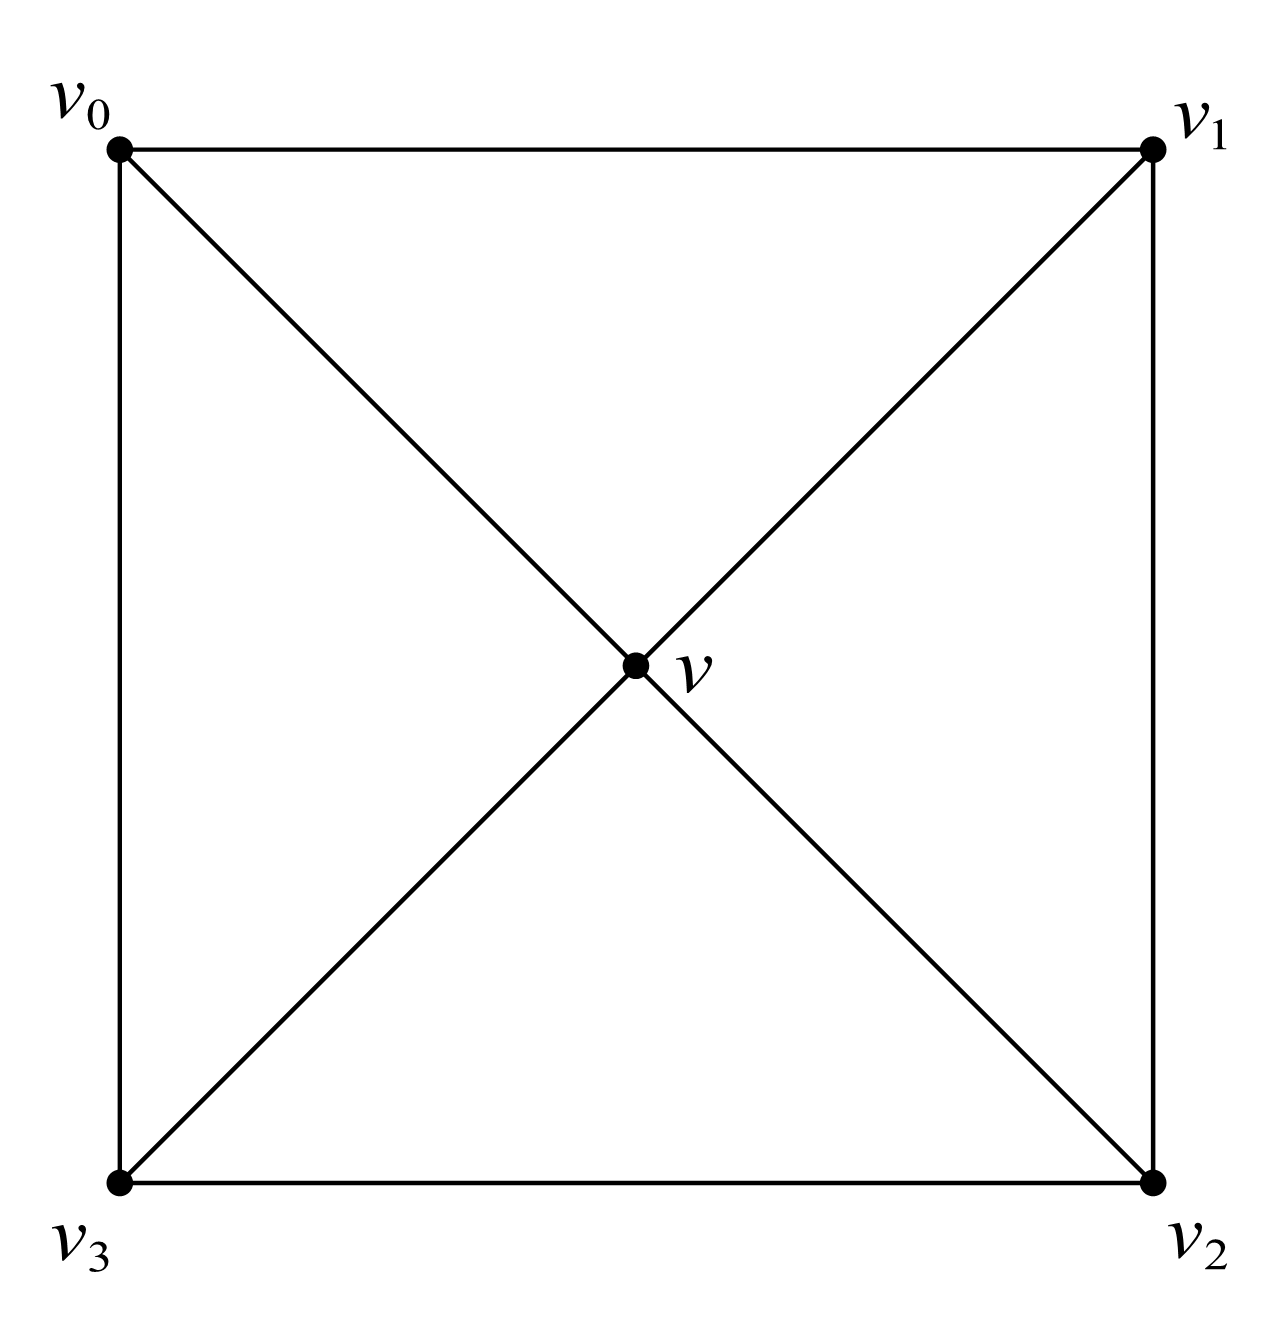
\includegraphics[width=0.2\linewidth]{figures/Sec8-1.png}
	\end{figure}
	首先考虑最简单的 $ p=2 $ 的情形:
	\[
		H_2(K,K_0)=C_2(K,K_0)=Z_2(K,K_0)=C_2(K),
	\]
	取 $ \bar{c}_2=\sum_{\dim\sigma=2}m_i\sigma_i\in Z_2(K,K_0) $, 那么
	\[
		\partial c_2\in C_1(K_0)\Longleftrightarrow m_1=m_2=m_3=m_4,
	\]
	于是 $ H_2(K,K_0)=Z_2(K,K_0)\cong\Z $.

	对于 $ p=1 $ 的情形, 情况就复杂了起来. 我们考虑
	\[
		\set{\bar{c}_1}\in H_1(K,K_0)\Longleftrightarrow\partial\bar{c}_1=0\Longleftrightarrow\partial c_1\in C_0(K_0),
	\]
	另一方面, 若 $ c_1\sim c_1' $ 使得 $ c_1' $ 被下面的复形承载,
	\begin{figure}[htbp]
		\centering
		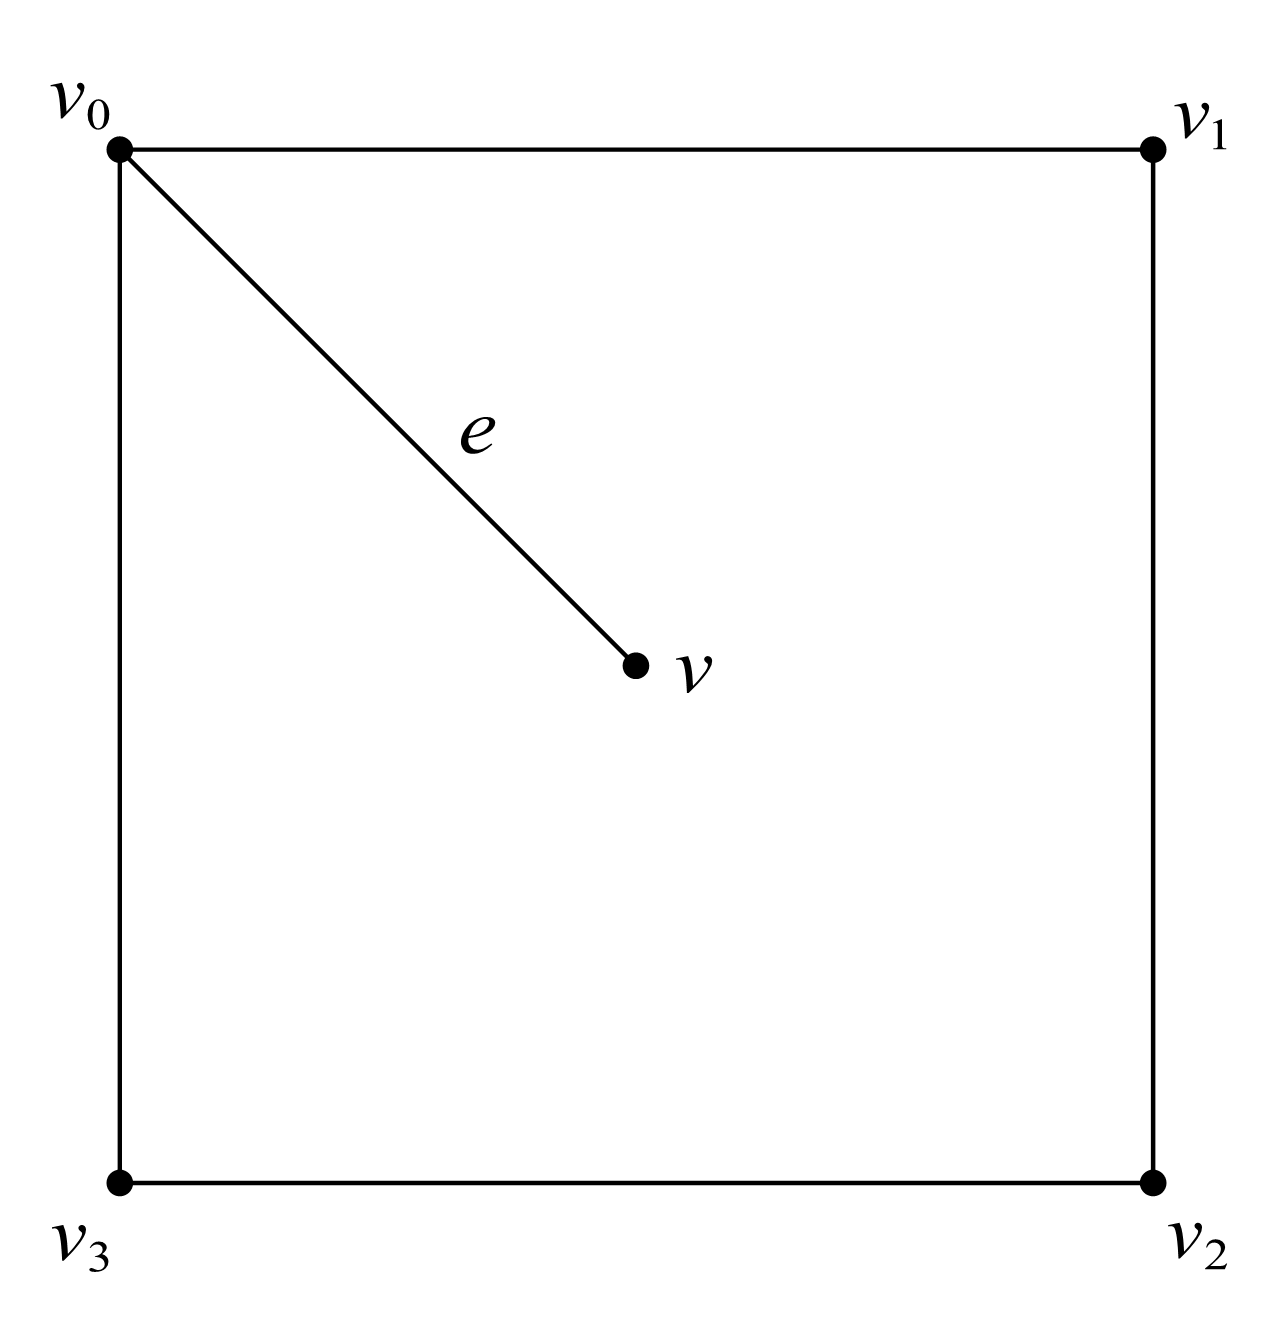
\includegraphics[width=0.2\linewidth]{figures/Sec8-2.png}
	\end{figure}
	那么
	\[
		\begin{aligned}
			\exists d\in C_2(K)\,(\partial d=c_1-c_1')&\Longrightarrow\partial\bar{d}=\baro{\partial d}=c_1-c_1'+C_1(K_0)\\
			&\Longrightarrow \partial^2\bar{d}=\partial c_1-\partial c_1'+C_0(K_0)\\
			&\Longrightarrow \partial^2\bar{d}=0=-\partial c_1'+C_0(K_0)\\
			&\Longrightarrow \partial c_1'\in C_0(K_0).
		\end{aligned}
	\]
	故 $ c_1' $ 也被 $ K_0 $ 承载. 则
	\[
		B_1(K,K_0)\ni\partial d=c_1-c_1'+C_1(K_0)=c_1+C_1(K_0)=\bar{c}_1\in Z_1(K,K_0),
	\]
	于是 $ H_1(K,K_0)=Z_1(K,K_0)/B_1(K,K_0)=0 $.

	对 $ p=0 $ 的情形, 因各 $ v_i $ 都有 $ v_i\in C_0(K_0) $ 成立, 于是
	\[
		\set{\bar{c}_0}\in H_0(K,K_0)\Longrightarrow\bar{c}_0=\ell v+C_0(K_0)\Longrightarrow\partial e=v-v_0,
	\]
	则
	\[
		B_0(K,K_0)\ni\partial(\ell\bar{e})=\ell(\partial\bar{e})=\ell v-\ell v_0+C_0(K_0)=\ell v+C_0(K_0)=\bar{c}_0\in Z_0(K,K_0),
	\]
	故 $ H_0(K,K_0)=Z_0(K,K_0)/B_0(K,K_0)=0 $.
\end{Example}

但幸运的是, 下面的引理使得我们计算相对同调群时无需每次都要走一次那么复杂的流程:

\begin{Theorem}[切除定理]
	设 $ K_0 $ 是 $ K $ 的子复形, 若开集 $ U\subset\abs{K_0} $ 使得
	\[
		\abs{K_0}\sm U=\abs{L_0},\qquad\abs{K}\sm U=\abs{L},
	\]
	这里 $ L_0 $ 是 $ K_0 $ 的子复形, $ L $ 是 $ K $ 的子复形, 则
	\[
		H_p(K,K_0)\cong H_p(L,L_0).
	\]
\end{Theorem}
\begin{Proof}
	因 $ L $ 是 $ K $ 的子复形, 于是
	\begin{center}
		\begin{tikzcd}
			C_p(L) \arrow[r, "\iota", hook] \arrow[rr, "\varphi", bend left] & C_p(K) \arrow[r, "\pi", two heads] & {C_p(K,K_0)} \\
			c \arrow[r, maps to]                                             & c \arrow[r, maps to]               & c+C_p(K_0)  
		\end{tikzcd}
	\end{center}
	由 $ \sigma\in K\sm K_0 $ 有 $ \set{\sigma_i} $ 是 $ C_p(K,K_0) $ 的基, 而 $ \sigma_i\in L $, 故 $ \varphi $ 是满的. 又因为 $ \ker\varphi=C_p(L_0) $, 故 $ \varphi $ 是单的. 于是 $ \varphi $ 是同构. 由第一同构定理可知 $ \varphi $ 诱导同构
	\[
		C_p(L)/C_p(L_0)\cong C_p(K,K_0).
	\]
	
	只需要 $ \partial $ 也被这一同构保持即可. 通过直接计算可以验证下图
	\begin{center}
		\begin{tikzcd}
			c+C_p(L_0) \arrow[rrr, maps to] \arrow[ddd, maps to] &                                                             &                                    & c+C_p(K_0) \arrow[ddd, maps to] \\
																 & {C_p(L,L_0)} \arrow[d, "\partial"] \arrow[r, "\bar\varphi"] & {C_p(K,K_0)} \arrow[d, "\partial"] &                                 \\
																 & {C_{p-1}(L,L_0)} \arrow[r, "\bar\varphi"]                   & {C_{p-1}(K,K_0)}                   &                                 \\
			\partial c+C_{p-1}(L_0) \arrow[rrr, maps to]         &                                                             &                                    & \partial c+C_{p-1}(K_0)        
		\end{tikzcd}
	\end{center}
	交换, 从而 $ H_p(L,L_0)\cong H_p(K,K_0) $.\qed
\end{Proof}

设 $ K_0 $ 是 $ K $ 的子复形, 那么 $ K_0\stackrel{\iota}{\hookrightarrow}K $ 诱导 $ H_p(K_0)\stackrel{\iota_*}{\hookrightarrow}H_p(K) $. 而 $ K $ 又可以看作复形对 $ (K,\emptyset) $, 于是 $ (K,\emptyset)\stackrel{j}{\hookrightarrow}(K,K_0) $ 又可以诱导 $ H_p(K)\stackrel{j_*}{\hookrightarrow}H_p(K,K_0) $. 于是我们得到一个序列
\begin{center}
	\begin{tikzcd}
		H_p(K_0) \arrow[r, "\iota_*", hook] & H_p(K) \arrow[r, "j_*", hook] & {H_p(K,K_0)} \arrow[r, "\partial_*"] & H_{p-1}(K_0)             \\
											&                               & \set{\bar{c}_p} \arrow[r, maps to]   & \set{\partial \bar{c}_p}
	\end{tikzcd}
\end{center}
在继续讨论它之前, 我们需要一点点其他的基础知识.

\subsection{正合序列}

之前我们讨论的是 $ R $--模上的正合列, 这里只需要讨论 $ \Z $--模, 或者说 Abel 群的正合列即可.

\begin{Definition}[正合序列]
	设 $ (A_i) $ 是一列 Abel 群, $ (\varphi_i) $ 是一列群同态, 若序列
	\begin{center}
		\begin{tikzcd}
			\cdots \arrow[r] & A_{i-1} \arrow[r, "\varphi_{i-1}"] & A_i \arrow[r, "\varphi_i"] & A_{i+1} \arrow[r, "\varphi_{i+1}"] & \cdots
		\end{tikzcd}
	\end{center}
	满足 $ \im\varphi_{i-1}=\ker\varphi_i $, 则称序列在 $ A_i $ 处\emph{正合}. 若它处处正合, 则称序列是一个\emph{正合序列}.
\end{Definition}

\begin{Proposition}
	正合列具有下面基本的性质. 这些性质验证起来都比较容易:
	\begin{enumerate}[(1)]
		\item 若序列 $ A_1\stackrel{\varphi}{\to}A_2\to 0 $ 正合, 则 $ \varphi $ 是满同态;
		\item 若序列 $ 0\to A_1\stackrel{\psi}{\to}A_2 $ 正合, 则 $ \psi $ 是单同态;
		\item 若序列 $ 0\to A_1\stackrel{\varphi}{\to}A_2\stackrel{\psi}{\to}A_3\to 0 $ 正合, 则 $ \psi\varphi=0 $.
		\item 短正合列
		\begin{center}
			\begin{tikzcd}
				A_1 \arrow[r, "\varphi"] & A_2 \arrow[r] & A_3 \arrow[r] & A_4 \arrow[r, "\psi"] & A_5
			\end{tikzcd}
		\end{center}
		诱导的序列
		\begin{center}
			\begin{tikzcd}
				0 \arrow[r] & \coker\varphi \arrow[r] & A_3 \arrow[r] & \ker\psi \arrow[r] & 0
			\end{tikzcd}
		\end{center}
		也是正合的.
	\end{enumerate}
\end{Proposition}

\begin{De-Pr}[分裂的正合列]
	称短正合列
	\begin{center}
		\begin{tikzcd}
			0 \arrow[r] & A_1 \arrow[r, "\varphi"] & A_2 \arrow[r, "\psi"] & A_3 \arrow[r] & 0
		\end{tikzcd}
	\end{center}
	是\emph{分裂}的, 若 $ A_2=\im\varphi\oplus B $. 此时 $ \psi|_B : B\to A_3 $ 是同构.
\end{De-Pr}
\begin{Proof}
	$ \psi|_B $ 是满同态容易得到, 下证它是单的. 设 $ b_1,b_2\in B $ 使得 $ \psi(b_1)=\psi(b_2) $, 则
	\[
		\begin{aligned}
			\psi(b_1)-\psi(b_2)=\psi(b_1-b_2)=0&\Longrightarrow b_1-b_2\in\ker\psi=\im\varphi\\
			&\Longrightarrow b_1-b_2\in\im\varphi\cap B\\
			&\Longrightarrow b_1-b_2=0.
		\end{aligned}
	\]
	从而 $ \psi|_B $ 是同构.\qed
\end{Proof}

此时对于分裂的正合列, 有图
\begin{center}
	\begin{tikzcd}
		0 \arrow[r] & A_1 \arrow[r, "\varphi"] \arrow[d, Rightarrow, no head] & A_2 \arrow[r, "\psi"] \arrow[d, "\theta"] & A_3 \arrow[r] \arrow[d, Rightarrow, no head] & 0 \\
		0 \arrow[r] & A_1 \arrow[r, "\iota", hook]                            & A_1\oplus A_3 \arrow[r, "\pi", two heads] & A_3 \arrow[r]                                & 0
	\end{tikzcd}
\end{center}
交换, 这即群扩张.

\begin{Proposition}[分裂正合列的判定]
	设
	\begin{center}
		\begin{tikzcd}
			0 \arrow[r] & A_1 \arrow[r, "\varphi"] & A_2 \arrow[r, "\psi"] & A_3 \arrow[r] & 0
		\end{tikzcd}
	\end{center}
	是短正合列, 下列叙述等价:
	\begin{enumerate}[(1)]
		\item 序列是分裂的;
		\item 存在 $ p : A_2\to A_1 $ 使得 $ p\varphi=\id_{A_1} $;
		\item 存在 $ j : A_3\to A_2 $ 使得 $ \psi j=\id_{A_3} $.
	\end{enumerate}
\end{Proposition}
\begin{proof}
	(1) $ \Rightarrow $ (2,3) : 只需注意到正合列等价于
	\begin{center}
		\begin{tikzcd}
			0 \arrow[r] & A_1 \arrow[r, "\varphi", shift left] & A_2 \arrow[r, "\psi", shift left] \arrow[l, "p", two heads, shift left] & A_3 \arrow[r] \arrow[l, "j", hook, shift left] & 0
		\end{tikzcd}
	\end{center}
	取 $ p : A_1\oplus A_3\twoheadrightarrow A_1 $ 是投影, 而 $ j : A_3\hookrightarrow A_1\oplus A_3 $ 是嵌入即可.

	(2) $ \Rightarrow $ (1) : 因对任意 $ x\in A_2 $, 有
	\[
		x=\varphi p(x)+(x-\varphi p(x))\in\im\varphi+\ker p,
	\]
	故只需验证这是直和. 取 $ x\in\im\varphi\cap\ker p $, 有
	\[
		x\in\im\varphi\Longrightarrow\exists y\in A_1\,(x=\varphi(y)),
	\]
	而
	\[
		x\in\ker p\Longrightarrow p(x)=p(\varphi(y))=y=0\Longrightarrow\varphi(y)=0
	\]
	这导出 $ x=0 $.

	(3) $ \Rightarrow $ (1) : 类似于上面, 对任意 $ x\in A_2 $, 有
	\[
		x=(x-j\psi(x))+j\psi(x)\in\ker\psi+j(A_3)
	\]
	只需验证这是直和. 取 $ x\in\ker\psi\cap j(A_3) $, 有
	\[
		x\in j(A_3)\Longrightarrow\exists y\in A_3(x=j(y)),
	\]
	而
	\[
		x\in\ker\psi\Longrightarrow y=\psi j(y)=\psi(x)=0\Longrightarrow j(y)=0
	\]
	这导出 $ x=0 $.\qed
\end{proof}

\begin{Corollary}
	若 $ A_3 $ 是自由 Abel 群, 则短正合列
	\begin{center}
		\begin{tikzcd}
			0 \arrow[r] & A_1 \arrow[r, "\varphi"] & A_2 \arrow[r, "\psi"] & A_3 \arrow[r] & 0
		\end{tikzcd}
	\end{center}
	分裂.
\end{Corollary}
\begin{Proof}
	取 $ A_3 $ 的一组基 $ \set{e_i} $, 则 $ \psi $ 是满同态, $ \psi^{-1}\ne\emptyset $. 取
	\[
		j : A_3\to A_2,\qquad e_i\mapsto a_i\in\psi^{-1}(e_i),
	\]
	则 $ \psi_j(e_i)=\psi(a_i)=e_i $, 这导出 $ \psi j=\id_{A_3} $.\qed
\end{Proof}

\begin{Definition}[链复形的短正合列]
	用 $ 0 $ 记零链, 设 $ \varphi : \CC\to\CD $ 和 $ \psi : \CD\to\CE $ 都是链映射, 称
	\begin{center}
		\begin{tikzcd}
			0 \arrow[r] & \CC \arrow[r, "\varphi"] & \CD \arrow[r, "\psi"] & \CE \arrow[r] & 0
		\end{tikzcd}
	\end{center}
	正合, 若对任何的 $ p\in\Z $ 都有
	\begin{center}
		\begin{tikzcd}
			0 \arrow[r] & C_p \arrow[r, "\varphi"] & D_p \arrow[r, "\psi"] & E_p \arrow[r] & 0
		\end{tikzcd}
	\end{center}
	正合.
\end{Definition}

下面的内容是有关正合列的三个重要结论, 分别是 zig--zag 引理, 五引理和蛇引理. 首先说明的就是 zig--zag 引理, 因为它的存在, 我们可以想到从短正合列出发构造长正合列. 而又因为正合列的性质, 我们可以从此出发构造相对同调群.

\begin{Lemma}[Zig--zag 引理]
	设
	\begin{center}
		\begin{tikzcd}
			0 \arrow[r] & \CC \arrow[r, "\varphi"] & \CD \arrow[r, "\psi"] & \CE \arrow[r] & 0
		\end{tikzcd}
	\end{center}
	正合, 则有长正合列
	\begin{center}
		\begin{tikzcd}
			\cdots \arrow[r] & H_p(\CC) \arrow[r, "\varphi_*"] & H_p(\CD) \arrow[r, "\psi_*"] & H_p(\CE) \arrow[r, "\partial_*"] & H_{p-1}(\CC) \arrow[r] & \cdots
		\end{tikzcd}
	\end{center}
\end{Lemma}
\begin{Proof}
	先明确 $ \partial_* $ 的定义: 对 $ \set{e_p}\in H_p(\CE) $, 为了确定 $ \partial_*(\set{e_p}) $, 我们使用以下的 `` 图追踪法 '' 来说明解决的思路. \textit{这种方法非常重要, 后面会反复使用.}
	\begin{center}
		\begin{tikzcd}
			0 \arrow[r] & C_p \arrow[r, "\varphi"] \arrow[d, "\partial_C"'] & D_p \arrow[r, "\psi"] \arrow[d, "\partial_D"'] & E_p \arrow[r] \arrow[d, "\partial_E"'] & 0 \\
			0 \arrow[r] & C_{p-1} \arrow[r, "\varphi"]                      & D_{p-1} \arrow[r, "\psi"]                      & E_{p-1} \arrow[r]                      & 0
		\end{tikzcd}
	\end{center}
	因 $ \psi $ 是满同态, 于是存在 $ d_p\in D_p $ 使得 $ \psi(d_p)=e_p $; 对 $ d_p $ 做边缘运算: 由 $ e_p\in Z_p(\CE) $ 可知
	\[
		\psi(\partial_D d_p)=\psi\partial_D d_p=\partial_E(\psi(d_p))=\partial_E e_p=0,
	\]
	于是 $ \partial_D d_p\in\ker\psi=\im\varphi $. 于是存在 $ c_{p-1}\in C_{p-1} $ 使得 $ \varphi(c_{p-1})=\partial_D d_p $, 还需要验证 $ c_{p-1}\in Z_{p-1}(\CC) $. 计算
	\[
		\varphi(\partial_C c_{p-1})=\partial_D\varphi(c_{p-1})=\partial_D(\partial_D d_p)=\partial_D^2 d_p=0,
	\]
	由 $ \varphi $ 是单同态可知 $ \partial_C c_{p-1}=0 $, 于是可以定义 $ \partial_*(\set{e_p})=\set{c_{p-1}} $.

	如此定义的 $ \partial_* $ 是良定义的. 为此, 另取 $ e_p'\in\set{e_p} $, 并且记类似得到的为 $ c_{p-1}'\in Z_{p-1}(\CC) $, 需证 $ \set{c_{p-1}}=\set{c_{p-1}'} $. 由 $ e_p\sim e_p' $ 可知存在 $ e_{p+1}\in E_{p+1} $ 使得 $ \partial_E e_{p+1}=e_p-e_p' $. 继续使用图追踪法
	\begin{center}
		\begin{tikzcd}
			0 \arrow[r] & C_p \arrow[r, "\varphi"] \arrow[d, "\partial_C"'] & D_p \arrow[r, "\psi"] \arrow[d, "\partial_D"'] & E_p \arrow[r] \arrow[d, "\partial_E"'] & 0 \\
			0 \arrow[r] & C_{p-1} \arrow[r, "\varphi"]                      & D_{p-1} \arrow[r, "\psi"]                      & E_{p-1} \arrow[r]                      & 0
		\end{tikzcd}
	\end{center}
	考虑
	\[
		\begin{aligned}
			\psi(d_p-d_p'-\partial_D d_{p+1})&=e_p-e_p'-\psi(\partial_D d_{p+1})\\
			&=e_p-e_p'-\partial_E(\psi(d_{p+1}))=e_p-e_p'-\partial_E e_{p+1}=0,
		\end{aligned}
	\]
	即 $ d_p-d_p'-\partial_D d_{p+1}\in\ker\psi=\im\varphi $, 故存在 $ c_p\in C_p $ 使得 $ \varphi(c_p)=d_p-d_p'-\partial_D d_{p+1} $, 计算
	\[
		\varphi(\partial_C c_p)=\partial_D(\varphi(c_p))=\partial_D(d_p-d_p'-\partial_D d_{p+1})=\partial_D d_p-\partial_D d_p'=\varphi(c_{p-1}-c_{p-1}'),
	\]
	因 $ \varphi $ 是单同态, $ \partial_C c_p=c_{p-1}-c_{p-1}' $, 即 $ c_{p-1}\sim c_{p-1}' $.

	下面验证序列在 $ H_p(\CE) $ 处的正合性, 即 $ \ker\partial_*=\im\psi_* $. 

	首先验证 $ \ker\partial_*\subset\im\psi_* $ : 任取 $ \set{e_p}\in\ker\partial_* $, 即 $ \set{c_{p-1}}=\partial_*(\set{e_p})=0 $. 取 $ d_p\in D_p $ 使得 $ \psi(d_p)=e_p $. 再取 $ c_p\in C_p $ 使得 $ \partial_C c_p=c_{p-1} $.
	\begin{center}
		\begin{tikzcd}
			0 \arrow[r] & C_p \arrow[r, "\varphi"] \arrow[d, "\partial_C"'] & D_p \arrow[r, "\psi"] \arrow[d, "\partial_D"'] & E_p \arrow[r] \arrow[d, "\partial_E"'] & 0 \\
			0 \arrow[r] & C_{p-1} \arrow[r, "\varphi"]                      & D_{p-1} \arrow[r, "\psi"]                      & E_{p-1} \arrow[r]                      & 0
		\end{tikzcd}
	\end{center}
	考虑 $ d_p-\varphi(c_p) $, 计算
	\[
		\partial_D(d_p-\varphi(c_p))=\partial_D d_p-\partial_D\varphi(c_p)=\partial_D d_p-\varphi(\partial_C c_p)=\partial_D d_p-\varphi(c_{p-1})=0,
	\]
	进而
	\[
		\psi_*(\set{d_p-\varphi(c_p)})=\set{\psi(d_p)-\psi\varphi(c_p)}=\set{\psi(d_p)}=\set{e_p}.
	\]
	即 $ \set{e_p}\in\im\psi_* $.

	再验证 $ \im\psi_*\subset\ker\partial_* $ : 任取 $ \set{e_p}\in\im\psi_* $, 则存在 $ \set{d_p'}\in H_p(\CD) $ 使得
	\[
		\set{\psi(d_p')}=\psi_*(\set{d_p'})=\set{e_p}.
	\]
	因 $ \partial_D d_p'=0 $, 有 $ e_p\sim\psi(d_p')=:e_p' $.
	\begin{center}
		\begin{tikzcd}
			0 \arrow[r] & C_p \arrow[r, "\varphi"] \arrow[d, "\partial_C"'] & D_p \arrow[r, "\psi"] \arrow[d, "\partial_D"'] & E_p \arrow[r] \arrow[d, "\partial_E"'] & 0 \\
			0 \arrow[r] & C_{p-1} \arrow[r, "\varphi"]                      & D_{p-1} \arrow[r, "\psi"]                      & E_{p-1} \arrow[r]                      & 0
		\end{tikzcd}
	\end{center}
	故 $ \partial_*(\set{e_p})=\partial_*(\set{e_p'})=0 $.

	序列在 $ H_p(\CD) $ 和在 $ H_{p-1}(\CC) $ 处的正合性类似可证.\qed
\end{Proof}

\begin{Theorem}
	设图
	\begin{center}
		\begin{tikzcd}
			0 \arrow[r] & \CC \arrow[r, "\varphi"] \arrow[d, "\alpha"'] & \CD \arrow[r, "\psi"] \arrow[d, "\beta"'] & \CE \arrow[r] \arrow[d, "\gamma"'] & 0 \\
			0 \arrow[r] & \CC' \arrow[r, "\varphi"]                      & \CD' \arrow[r, "\psi"]                     & \CE' \arrow[r]                      & 0
		\end{tikzcd}
	\end{center}
	交换, 那么图
	\begin{center}
		\begin{tikzcd}
			{} \arrow[r] & H_p(\CC) \arrow[r, "\varphi_*"] \arrow[d, "\alpha_*"'] & H_p(\CD) \arrow[r, "\psi_*"] \arrow[d, "\beta_*"'] & H_p(\CE) \arrow[r, "\partial_*"] \arrow[d, "\gamma_*"'] & H_{p-1}(\CC) \arrow[r] \arrow[d, "\alpha_*"'] & {} \\
			{} \arrow[r] & H_p(\CC') \arrow[r, "\varphi_*'"]                      & H_p(\CD') \arrow[r, "\psi_*'"]                     & H_p(\CE') \arrow[r, "\partial_*'"]                      & H_{p-1}(\CC') \arrow[r]                       & {}
		\end{tikzcd}
	\end{center}
	也交换.
\end{Theorem}
\begin{Proof}
	考虑中间三个方块的交换性. 前两个方块的交换性是简单的, 以第一个为例. 取 $ \set{c_p}\in H_p(\CC) $, 有
	\[
		\beta_*\varphi_*(\set{c_p})=\set{\beta\varphi(c_p)}=\set{\varphi'\alpha(c_p)}=\varphi_*'\alpha_*(\set{c_p}),
	\]
	故第一个方块交换.

	主要讨论第三个方块的交换性, 取 $ \set{e_p}\in H_p(\CE) $. 则存在 $ c_{p-1} $ 和 $ d_p $ 使得 $ \varphi(c_{p-1})=\partial_D d_p $, $ \psi(d_p)=e_p $. 需要验证 $ \alpha_*\partial_*(\set{e_p})=\partial_*'\gamma_*(\set{e_p}) $.
	\begin{figure}[htbp]
		\centering
		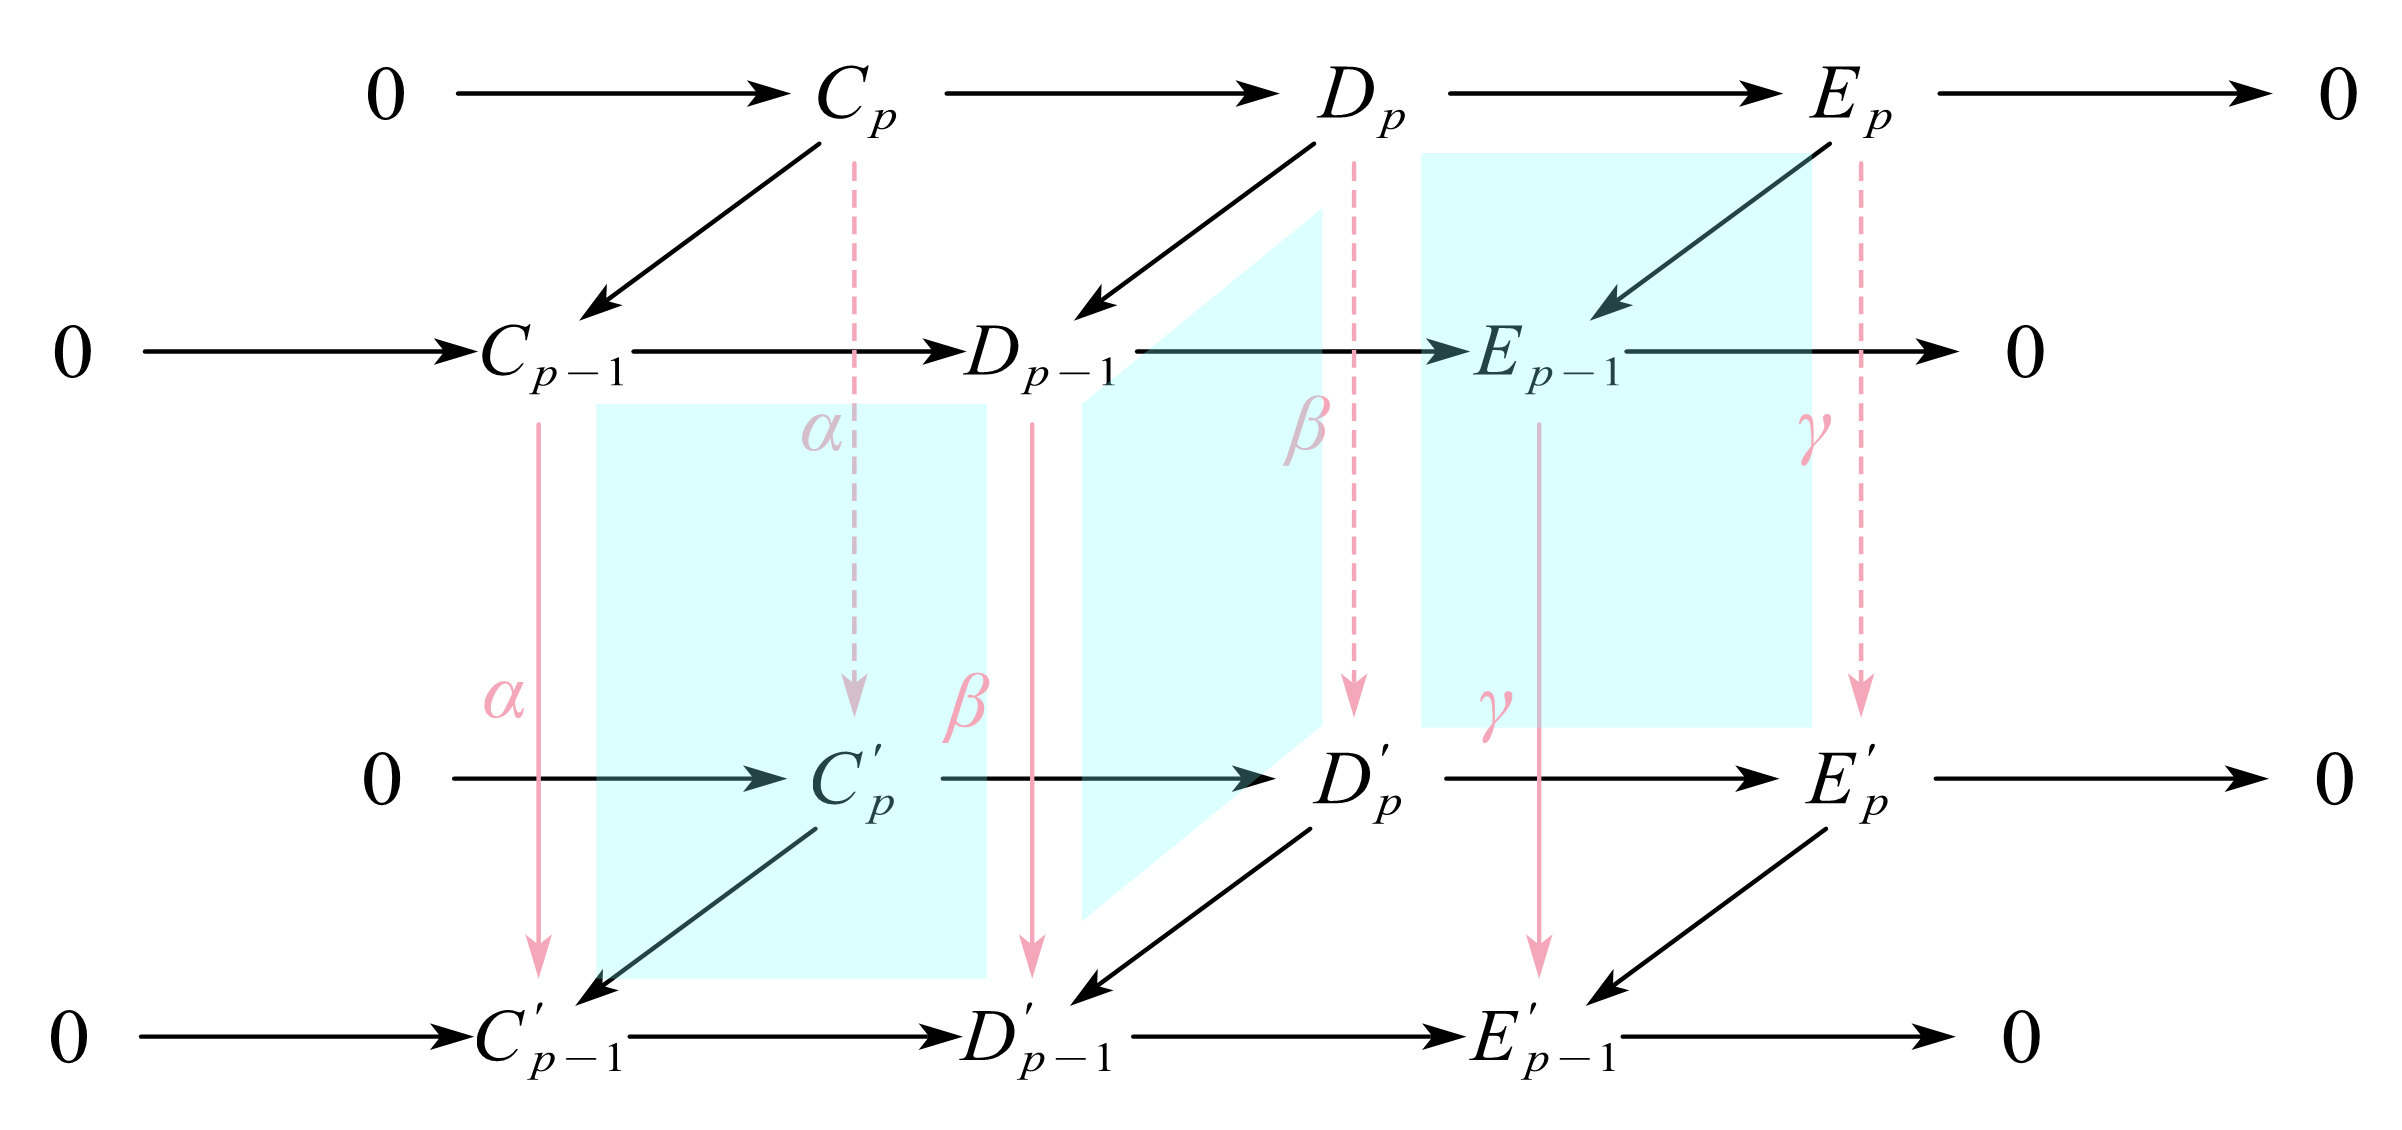
\includegraphics[width=0.55\linewidth]{figures/Sec8-4.png}
	\end{figure}\\
	由
	\[
		\alpha_*\partial_*(\set{e_p})=\alpha_*(\set{c_{p-1}})=\set{\alpha(c_{p-1})},
	\]
	和
	\[
		\partial_*\gamma_*(\set{e_p})=\partial_*'(\set{\gamma(e_p)}).
	\]
	本质上只需要验证 $ \partial_*'(\set{\gamma(e_p)})=\set{\alpha(c_{p-1})} $ 即可. 注意到淡蓝色标出的方块都是交换的, 由
	\[
		\psi'\beta(d_p)=\gamma\psi(d_p)=\gamma(e_p)
	\]
	和
	\[
		\varphi'\alpha(c_{p-1})=\beta\varphi(c_{p-1})=\beta(\partial_D d_p)=\partial_D'\beta(d_p).
	\]
	从而有 $ \partial_*'(\set{\gamma(e_p)})=\set{\alpha(c_{p-1})} $.\qed
\end{Proof}

\begin{Lemma}[五引理]
	设 $ A_i $, $ B_j $ 是 Abel 群, 水平的序列都是正合的.
	\begin{center}
		\begin{tikzcd}
			A_1 \arrow[r, "\alpha_1"] \arrow[d, "f_1"] & A_2 \arrow[r, "\alpha_2"] \arrow[d, "f_2"] & A_3 \arrow[r, "\alpha_3"] \arrow[d, "f_3"] & A_4 \arrow[r, "\alpha_4"] \arrow[d, "f_4"] & A_5 \arrow[d, "f_5"] \\
			B_1 \arrow[r, "\beta_1"]                   & B_2 \arrow[r, "\beta_2"]                   & B_3 \arrow[r, "\beta_3"]                   & B_4 \arrow[r, "\beta_4"]                   & B_5                 
		\end{tikzcd}
	\end{center}
	那么
	\begin{enumerate}
		\item 若 $ f_1 $ 是满的, $ f_2,\ f_4 $ 是单的, 则 $ f_3 $ 是单的;
		\item 若 $ f_5 $ 是单的, $ f_2,\ f_4 $ 是满的, 则 $ f_3 $ 是满的;
		\item 若 $ f_1 $ 是满的, $ f_5 $ 是单的, $ f_2,\ f_4 $ 是同构, 则 $ f_3 $ 是同构.
	\end{enumerate}
\end{Lemma}
\begin{Proof}
	(1) 使用图追踪法:
	\begin{center}
		\begin{tikzcd}
			A_1 \arrow[r, "\alpha_1"] \arrow[d, "f_1"] & A_2 \arrow[r, "\alpha_2"] \arrow[d, "f_2"] & A_3 \arrow[r, "\alpha_3"] \arrow[d, "f_3"] & A_4 \arrow[r, "\alpha_4"] \arrow[d, "f_4"] & A_5 \arrow[d, "f_5"] \\
			B_1 \arrow[r, "\beta_1"]                   & B_2 \arrow[r, "\beta_2"]                   & B_3 \arrow[r, "\beta_3"]                   & B_4 \arrow[r, "\beta_4"]                   & B_5                 
		\end{tikzcd}
	\end{center}
	那么取 $ x\in\ker f_3 $, 由 $ f_4 $ 是单同态可知 $ \alpha_3(x)=0 $, 而 $ w $ 和 $ f_1(v) $ 的存在性由正合性得到. 这里 $ v $ 的存在性因 $ f_1 $ 是满同态.

	由图表的交换性, 有 $ f_2(w)=f_2(\alpha_1(v)) $, 由 $ f_2 $ 是单同态, 有 $ w=\alpha_1(v) $. 从而
	\[
		x=\alpha_2(w)=\alpha_2\alpha_1(v)=0,
	\]
	其中 $ \alpha_2\alpha_1=0 $ 由正合性得到, 即 $ f_3 $ 是单的.

	(2) 使用图追踪法:
	\begin{center}
		\begin{tikzcd}
			A_1 \arrow[r, "\alpha_1"] \arrow[d, "f_1"] & A_2 \arrow[r, "\alpha_2"] \arrow[d, "f_2"] & A_3 \arrow[r, "\alpha_3"] \arrow[d, "f_3"] & A_4 \arrow[r, "\alpha_4"] \arrow[d, "f_4"] & A_5 \arrow[d, "f_5"] \\
			B_1 \arrow[r, "\beta_1"]                   & B_2 \arrow[r, "\beta_2"]                   & B_3 \arrow[r, "\beta_3"]                   & B_4 \arrow[r, "\beta_4"]                   & B_5                 
		\end{tikzcd}
	\end{center}
	任取 $ y\in B_3 $, $ w\in A_4 $ 的存在性由 $ f_4 $ 是满同态得到. 由正合性可知 $ \beta_4\beta_3=0 $, 而 $ f_5 $ 是单同态, 于是
	\[
		w\in\ker\alpha_4=\im\alpha_3,
	\]
	那么 $ x $ 的存在性也得到了. 由图表的交换性可得
	\[
		\beta_3f_3(x)=f_4\alpha_3(x)=\beta_3(y),
	\]
	那么 $ y-f_3(x)\in\ker\beta_3=\im\beta_2 $, 故 $ z $ 的存在性得到. 而 $ v\in X_2 $ 的存在性由 $ f_2 $ 是满同态得到. 此时
	\[
		f_3(\alpha_2(v)+x)=f_3\alpha_2(v)+f_3(x)=y-f_3(x)+f_3(x)=y,
	\]
	即 $ y\in\im f_3 $.

	(3) 是 (1) 和 (2) 的直接推论.
\end{Proof}

\begin{Lemma}[蛇引理]
	设下图中水平序列均是正合的, $ \alpha,\ \beta,\ \gamma $ 是同态,
	\begin{center}
		\begin{tikzcd}
			0 \arrow[r] & A \arrow[r] \arrow[d, "\alpha"'] & B \arrow[r] \arrow[d, "\beta"'] & C \arrow[r] \arrow[d, "\gamma"'] & 0 \\
			0 \arrow[r] & D \arrow[r]                      & E \arrow[r]                     & F \arrow[r]                      & 0
		\end{tikzcd}
	\end{center}
	则序列
	\begin{center}
		\begin{tikzcd}
			0 \arrow[r] & \ker\alpha \arrow[r] & \ker\beta \arrow[r] & \ker\gamma \arrow[r] & \coker\alpha \arrow[r] & \coker\beta \arrow[r] & \coker\gamma \arrow[r] & 0
		\end{tikzcd}
	\end{center}
	是正合的.
\end{Lemma}
\begin{Proof}
	我们考虑下面的交换图
	\begin{center}
		\begin{tikzcd}
			0 \arrow[r] & \ker\alpha \arrow[r] \arrow[d]              & \ker\beta \arrow[r] \arrow[d]           & \ker\gamma \arrow[d]             &   \\
			0 \arrow[r] & A \arrow[r, "\varphi"] \arrow[d, "\alpha"'] & B \arrow[r, "\psi"] \arrow[d, "\beta"'] & C \arrow[r] \arrow[d, "\gamma"'] & 0 \\
			0 \arrow[r] & D \arrow[d] \arrow[r, "\varphi'"]           & E \arrow[r, "\psi'"] \arrow[d]          & F \arrow[r] \arrow[d]            & 0 \\
						& \coker\alpha \arrow[r]                      & \coker\beta \arrow[r]                   & \coker\gamma \arrow[r]           & 0
		\end{tikzcd}
	\end{center}
	对它做图追踪. 注意到所有水平方向的序列都是正合的, 所有竖直方向的序列也是正合的, 这直接导出所求证的序列在 $ \ker\beta $ 和 $ \coker\beta $ 处正合.

	下面的证明主要分三步.

	(1) 首先, 我们构造 $ \delta : \ker\gamma\to\coker\alpha $. 取 $ c\in\ker\gamma $, 因 $ B\to C\to 0 $ 正合, 故 $ B\to C $ 是满同态, 即
	\[
		\exists b\in B\,(\psi(b)=c).
	\]
	再设 $ e=\beta(b) $, 由图表的交换性由 $ \psi'(e)=0 $, 故 $ e\in\ker\psi'=\im\varphi' $. 那么存在 $ d\in D $ 使得 $ \varphi'(d)=e $, 并记 $ d $ 在 $ D\to\coker\alpha $ 下的像为 $ \bar{d} $. 于是可以定义 $ \delta(c)=d $.

	(2) 再验证序列在 $ \ker\gamma $ 和 $ \coker\alpha $ 处的正合性. 首先考虑 $ \ker\gamma $ 处, 序列
	\begin{center}
		\begin{tikzcd}
			\ker\beta \arrow[r] & \ker\gamma \arrow[r, "\delta"] & \coker\alpha
		\end{tikzcd}
	\end{center}
	的正合性需要验证 $ \ker\delta=\im[\ker\beta\to\ker\gamma] $. 若 $ c\in\ker\gamma $ 使得 $ \delta(c)=\bar{d}=0 $, 由 $ \delta $ 的构造过程可知存在一个 $ b'\in B $ 使得 $ b-b'\in\ker\beta $. 而 $ A\to B\to C $ 正合, 故 $ c\in\im[\ker\beta\to\ker\gamma] $. 于是 $ \ker\gamma $ 处是正合的.

	再考虑 $ \coker\alpha $ 处, 序列
	\begin{center}
		\begin{tikzcd}
			\ker\gamma \arrow[r, "\delta"] & \coker\alpha \arrow[r] & \coker\beta
		\end{tikzcd}
	\end{center}
	的正合性需要验证 $ \ker[\coker\alpha\to\coker\beta]=\im\delta $. 若 $ d\in D $ 在 $ D\to\coker\alpha $ 下的像为 $ \bar{d} $, 则 $ \bar{d}\in\ker[\coker\alpha\to\coker\beta] $ 当且仅当存在 $ b\in B $ 使得 $ \beta(b)=\varphi'(d) $. 由图表的交换性可知
	\[
		\gamma\psi(b)=\beta\psi'(\varphi(d))=0.
	\]
	于是 $ \psi(b)\in\ker\gamma $. 由 $ \delta $ 的构造可知
	\[
		\bar{d}=0\Longleftrightarrow\exists c\in\ker\gamma\,(\delta(c)=\bar{d}).
	\]
	于是 $ d\in\im\delta $, 故序列在 $ \coker\alpha $ 处正合.

	(3) 因出入 $ 0 $ 的同态必为零同态, 故序列在 $ \ker\alpha $ 和 $ \coker\gamma $ 处的正合性显然.\qed
\end{Proof}

一个更简单的办法是直接将竖列看作是链复形, 只有 $ \partial_1 $ 分别是 $ \alpha,\beta,\gamma $, 其他的边缘算子均为零. 此时注意到蛇引理所求证的正合序列无非是 zig--zag 引理导出的长正合列, 而证明中构造的 $ \delta $ 无非是 zig--zag 引理中的 $ \partial_* $.

\subsection{Mayer--Vietoris 序列}

考虑连续映射 $ f : (\abs{K},\abs{K_0})\to(\abs{L},\abs{L_0}) $, 它可以诱导长正合列的同态
\begin{center}
	\begin{tikzcd}
		{} \arrow[r] & H_p(\abs{K_0}) \arrow[r] \arrow[d, "f_*"'] & H_p(\abs{K}) \arrow[r] \arrow[d, "f_*"'] & {H_p(\abs{K},\abs{K_0})} \arrow[r] \arrow[d, "f_*"'] & H_{p-1}(\abs{K_0}) \arrow[r] \arrow[d, "f_*"'] & {} \\
		{} \arrow[r] & H_p(\abs{L_0}) \arrow[r]                   & H_p(\abs{L}) \arrow[r]                   & {H_p(\abs{L},\abs{L_0})} \arrow[r]                   & H_{p-1}(\abs{L_0}) \arrow[r]                   & {}
	\end{tikzcd}
\end{center}

类似于 van Kampen 定理的想法, 对 $ K=K_1\cup K_2 $, 且 $ K_0=K_1\cap K_2 $ 是单纯复形. 那么
\begin{center}
	\begin{tikzcd}
		& K_1 \arrow[rd, "k", hook]  &   \\
K_0 \arrow[ru, "\iota", hook] \arrow[rd, "j"', hook] \arrow[rr, "m", hook] &                            & K \\
		& K_2 \arrow[ru, "l"', hook] &  
	\end{tikzcd}
\end{center}
考虑链复形的嵌入
\begin{center}
	\begin{tikzcd}
		0 \arrow[r] & \CC(K_0) \arrow[r, "\varphi", hook] & \CC(K_1)\oplus\CC(K_2) \arrow[r, "\psi", two heads] & \CC(K) \arrow[r] & 0 \\
					& c \arrow[r, maps to]                & {(\iota_\sharp(c),j_\sharp(c))}                     &                  &   \\
					&                                     & {(c_1,-c_2)} \arrow[r, maps to]                     & c_1+c_2          &  
	\end{tikzcd}
\end{center}
那么 $ \varphi $ 是单射, $ \psi $ 是满射, 那么 $ \varphi,\ \psi $ 是链映射.

\textit{只是一个给自己的小提示, 在链复形中一定要记得验证 $ \varphi,\psi $ 与 $ \partial $ 的交换性, 即图}
\begin{center}
	\begin{tikzcd}
		C_p(K_0) \arrow[r, "\varphi", hook] \arrow[d, "\partial"'] & C_p(K_1)\oplus C_p(K_2) \arrow[d, "\partial"] \\
		C_{p-1}(K_0) \arrow[r, "\varphi", hook]                    & C_{p-1}(K_1)\oplus C_{p-1}(K_2)              
	\end{tikzcd}
\end{center}
下面验证序列的正合性. 即验证 $ \ker\psi=\im\varphi $. 这里 $ \im\varphi\subset\ker\psi $ 是显然的, 这因 $ \psi\varphi=0 $. 下面验证 $ \ker\psi\subset\im\varphi $: 取 $ c=(c_1,c_2)\in\ker\psi $, 则
\[
	\psi(c)=c_1+c_2=0\Longrightarrow c_1=-c_2\in\CC(K_1)\cap\CC(K_2)=\CC(K_1\cap K_2).
\]
记 $ c_1=-c_2=c'\in\CC(K_1\cap K_2) $, 则
\[
	\varphi(c')=(c',-c')=(c_1,c_2)=c,
\]
故 $ c\in\im\varphi $.

\begin{De-Th}[Mayer--Vietoris 序列]
	设 $ K $ 是复形, $ K_1,\ K_2 $ 是 $ K $ 的子复形, 满足 $ K=K_1\cup K_2 $. 记 $ K_0=K_1\cap K_2 $, 则存在长正合序列
	\begin{center}
		\begin{tikzcd}
			\cdots \arrow[r] & H_p(K_0) \arrow[r] & H_p(K_1)\oplus H_p(K_2) \arrow[r] & H_p(K) \arrow[r] & H_{p-1}(K_0) \arrow[r] & \cdots
		\end{tikzcd}
	\end{center}
	称作是 $ (K_1,K_2) $ 的 \emph{Mayer--Vietoris 序列}.
\end{De-Th}
\begin{Proof}
	在上述讨论中已经说明了序列是正合的, 于是它导出同调正合序列.\qed
\end{Proof}

Mayer--Vietoris 序列说明了两个复形的一点并导出的同调群恰为它们的直和: 取 $ X=A\cup B $, 其中 $ A\cap B=\set{v} $, 那么在 $ p>0 $ 时列出 Mayer--Vietoris 序列
\begin{center}
	\begin{tikzcd}
		\cdots \arrow[r] & \tilde{H}_p(v) \arrow[r] & \tilde{H}_p(A)\oplus\tilde{H}_p(B) \arrow[r] & \tilde{H}_p(X) \arrow[r] & \tilde{H}_{p-1}(v) \arrow[r] & \cdots
	\end{tikzcd}
\end{center}
于是 $ \tilde{H}_p(X)\cong\tilde{H}_p(A)\oplus\tilde{H}_p(B) $.

至此, 我们可以完全使用公理化的方式来描述同调论: 下面我们约定提到的空间都是可以三角剖分的拓扑空间. 考虑下面的一组公理:
\begin{enumerate}
	\item $ \id : X\to X $ 应当诱导出恒等映射 $ \id_* $.
	\item 若 $ X\stackrel{f}{\to} Y\stackrel{g}{\to} Z $, 则 $ (gf)_*=g_*f_* $.
	\item 对 $ f : (X,A)\to (Y,B) $, 图
	\begin{center}
		\begin{tikzcd}
			{H_p(X,A)} \arrow[r, "f_*"] \arrow[d, "\partial_*"] & {H_p(Y,B)} \arrow[d, "\partial_*"] \\
			H_p(A) \arrow[r, "(f|_A)_*"]                        & H_p(B)                            
		\end{tikzcd}
	\end{center}
	交换.
	\item 对复形对 $ (X,A) $, 序列
	\begin{center}
		\begin{tikzcd}
			\cdots \arrow[r] & H_p(A) \arrow[r, "\iota_*"] & H_p(X) \arrow[r, "j_*"] & {H_p(X,A)} \arrow[r, "\partial_*"] & H_{p-1}(A) \arrow[r] & \cdots
		\end{tikzcd}
	\end{center}
	是正合的, 其中 $ \iota : X\to A $ 和 $ j : (X,\emptyset)\to(X,A) $ 是嵌入.
	\item (同伦公理) 若 $ f\simeq g : X\to Y $, 则 $ f_*=g_* $.
	\item (切除公理) 给定复形对 $ (X,A) $, 设开集 $ U $ 满足 $ \bar{U}\subset\mathrm{Int}\,A $, 则 $ H_p(X,A)\cong H_p(X\sm U,A\sm U) $.
	\item (维数公理) $ \tilde{H}_p(\mathrm{pt})=0 $.
	\item (紧支撑公理) 若 $ \alpha\in H_p(X,A) $, 则存在 $ X_0,A_0 $ 是紧的, 同态 $ \iota : (X_0,A_0)\to (X,A) $, 使得 $ \alpha\in\im[\iota_* : H_p(X_0,A_0)\to H_p(X,A)] $.
\end{enumerate}

在这里如果去掉维数公理, 则称前六条公理构成的同调为\emph{广义同调}. 上述公理称作是单纯同调的 \emph{Eilenburg--Steenrod 公理}.

\subsection{奇异链复形}

奇异同调导出的思路类似于在对基本群的讨论中, 将道路视作映射 $ \sigma : I\to X $, 接下来我们将单形视作映射 $ T : \Delta_p\to X $.

在空间 $ \R^\N $ 上, 有几何独立的点
\[
	\begin{aligned}
		\varepsilon_0&=(0,0,\dots,0,\dots)\\
		\varepsilon_1&=(1,0,\dots,0,\dots)\\
		&\quad\vdots\\
		\varepsilon_p&=(0,0,\dots,1,\dots)\\
	\end{aligned}
\]
则 $ \set{\varepsilon_0,\dots,\varepsilon_p} $ 确定一个单形 $ \Delta_p $.

\begin{Definition}[奇异单形]
	记号同上面的约定, 称连续映射 $ T : \Delta_p\to X $ 是一个 $ p $ 维\emph{奇异单形}, 此时 $ p $ 维奇异单形全体即为 $ C(\Delta_p,X) $. 并记以 $ C(\Delta_p,X) $ 中元素为生成元产生的自由 Abel 群为 $ S_p(X) $, 称作 $ X $ 的 $ p $ 维\emph{奇异链群}.
\end{Definition}

对 $ c : C(\Delta_p,X)\to\Z $, $ T\mapsto c(T) $, 它至少应当满足 $ c(-T)=-c(T) $, 且仅对 $ C(\Delta_p,X) $ 中有限个元素使得 $ c(T)\ne 0 $.

但将单形看作映射带来的问题是, 如何刻画 $ T $ 的 $ p $ 维面. 此时已经没有足够好的几何直观, 为此, 我们考虑比较简单的奇异单形:

\begin{Definition}[线性奇异单形]
	设 $ a_0,\dots,a_p $ 是 $ \R^\N $ 中的任意 $ p+1 $ 个点, 这 $ p+1 $ 个点未必几何独立. 存在仿射变换
	\[
		\ell : \Delta_p\to\R^\N,\qquad \varepsilon_i\mapsto a_i\,(i=0,1,\dots,p)
	\]
	则对 $ x=(x_1,x_2,\dots,x_p,0,\dots) $, 有
	\[
		\ell(x)=a_0+\sum_{i=1}^p(a_i-a_0)x_i,
	\]
	记这一仿射变换 $ \ell $ 为 $ \ell(a_0,\dots,a_p) $, 并称作 $ \R^\N $ 中的\emph{线性奇异单形}.
\end{Definition}

特别地, 若 $ \varepsilon_i=a_i $, 那么此时 $ \ell(\varepsilon_0,\dots,\varepsilon_p) : \Delta_p\hookrightarrow\R^\N $ 是一个到上的同胚, 此时 $ \ell(\varepsilon_0,\dots,\varepsilon_p) $ 就是嵌入同胚. 称
\[
	\ell(\varepsilon_0,\dots,\hat{\varepsilon}_i,\dots,\varepsilon_p) : \Delta_{p-1}\hookrightarrow \R^\N
\]
是 $ \ell(\varepsilon_0,\dots,\varepsilon_p) $ 的第 $ i $ 个 $ p-1 $ 维面. 为了方便, 将这一线性奇异单形记作 $ \ell_{i,p} $.

\begin{figure}[htbp]
	\centering
	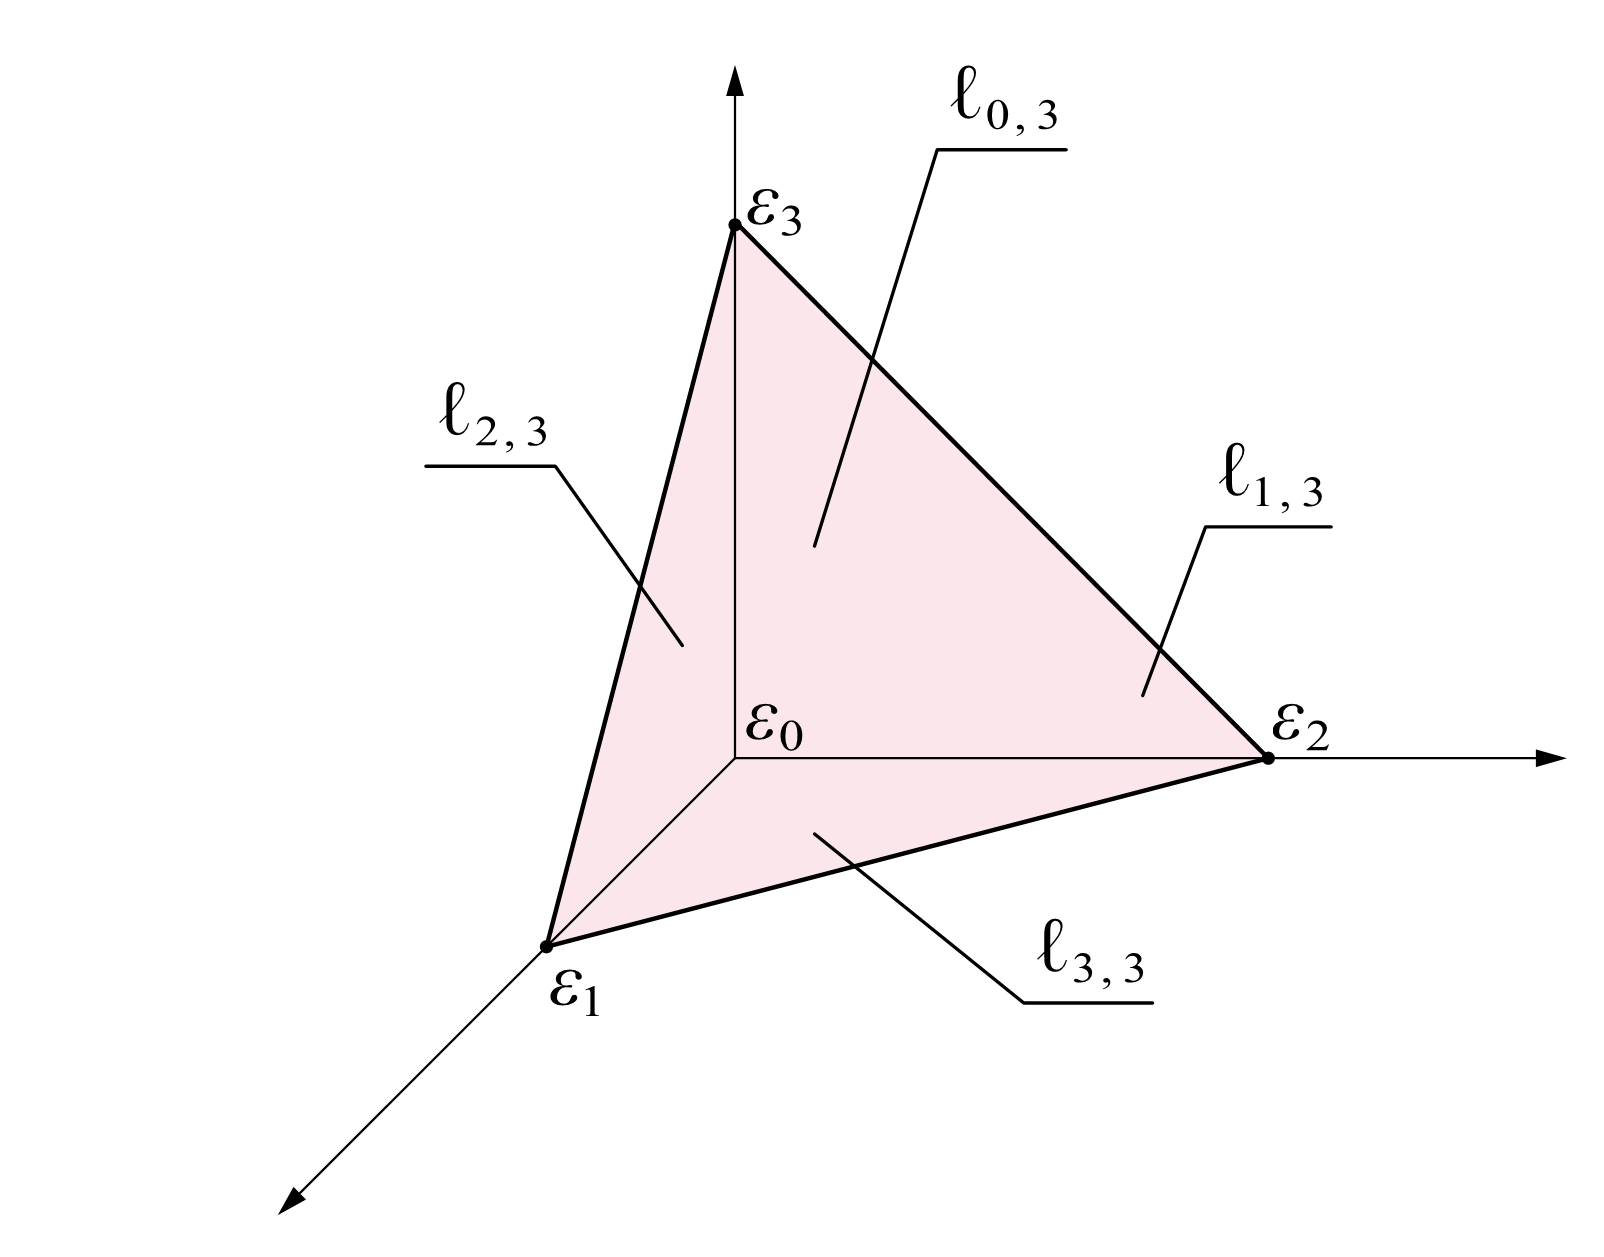
\includegraphics[width=0.4\linewidth]{figures/Sec10-1.png}
	%\caption{$ \Delta_3 $ 的所有 2 维面}
\end{figure}

\begin{Definition}[奇异单形的边界]
	对 $ T_p : \Delta_p\to X $, 称
	\[
		T_p\circ\ell_{i,p} : \Delta_{p-1}\to X
	\]
	是 $ T_p $ 的第 $ i $ 个 $ p-1 $ 维面, 故可定义
	\[
		\partial T_p:=\sum_{i=0}^p(-1)^iT_p\circ\ell_{i,p}
	\]
	是 $ T_p $ 的\emph{边界}.
\end{Definition}

连续映射 $ f : X\to Y $ 可以诱导链映射
\[
	f_\sharp : S_p(X)\to S_p(Y),\qquad T\mapsto f_\sharp(T):=f\circ T.
\]

\begin{Proposition}
	设 $ f\in C(X,Y) $, 则 $ f_\sharp\partial=\partial f_\sharp $.
\end{Proposition}
\begin{Proof}
	直接计算
	\[
		f_\sharp\partial T=f_\sharp\left( \sum_{i=0}^p(-1)^iT\circ\ell_{i,p} \right)=\sum_{i=0}^p(-1)^if\circ (T\circ\ell_{i,p})
	\]
	和
	\[
		\partial f_\sharp(T)=\partial(f\circ T)=\sum_{i=0}^p(-1)^i(f\circ T)\circ\ell_{i,p},
	\]
	得到 $ f_\sharp\partial=\partial f_\sharp $.\qed
\end{Proof}

\begin{Theorem}
	$ \partial^2=0 $.
\end{Theorem}
\begin{Proof}
	因 $ T\in C(\Delta_p,X) $ 可以诱导
	\[
		T_\sharp : S_p(\Delta_p)\to S_p(X),\qquad \ell(\varepsilon_0,\dots,\varepsilon_p)\mapsto T\circ\ell(\varepsilon_0,\dots,\varepsilon_p)=T.
	\]
	则对 $ T\in C(\Delta_p,X) $, 计算
	\[
		\begin{aligned}
			\partial^2T&=\partial^2T_\sharp\ell(\varepsilon_0,\dots,\varepsilon_p)\\
			&=T_\sharp\partial^2\ell(\varepsilon_0,\dots,\varepsilon_p)\\
			&=T_\sharp\partial\left( \sum_{i=0}^p(-1)^i\ell(\varepsilon_0,\dots,\varepsilon_p)\ell_{i,p} \right)\\
			&=T_\sharp\partial\left( \sum_{i=0}^p(-1)^i\ell_{i,p} \right)\\
			&=0.
		\end{aligned}
	\]
	其中倒数第二个等号因 $ \ell(\varepsilon_0,\dots,\varepsilon_p) $ 实际上就是 $ \id $.
\end{Proof}

由此我们构造了自由 Abel 群 $ S_p(X) $ 和其上的边缘算子 $ \partial $, 并且它们的性质和在单纯同调中的链复形满足的条件是相同的, 于是可以类似地定义链复形如下:

\begin{Definition}[奇异链复形]
	称 $ \CS(X):=\set{(S_p(X),\partial)} $ 是 $ X $ 的\emph{奇异链复形}, 由此可以定义同调群
	\[
		H_p(\CS(X))=H_p(X)=\ker\partial_p/\im\partial_{p+1},
	\] 
	并且记号与单纯同调中保持相同, 仍有 $ Z_p(X) $ 和 $ B_p(X) $.
\end{Definition}

类似地, $ f\in C(X,Y) $ 不仅可以诱导奇异链复形之间的链映射 $ f_\sharp : \CS(X)\to \CS(Y) $, 还可以诱导奇异同调群的同态 $ f_* : H_p(X)\to H_p(Y) $.

\begin{Theorem}
	$ H_* : X\mapsto H_p(X),\ f\mapsto f_* $ 是一个从 $ \category{Top} $ 到 $ \category{Grp} $ 的函子.
\end{Theorem}
\begin{Proof}
	只需要说明两点, 首先是恒等映射 $ \id_X : X\to X $ 诱导出的 $ (\id_X)_* $ 应当仍是恒等映射, 这是显然的. 只需要证明若 $ X\stackrel{f}{\to}Y\stackrel{g}{\to}Z $, 成立 $ (gf)_*=g_*f_* $ 即可. 为此, 只需要在链层面证明: 这因
	\[
		(gf)_\sharp(T)=(gf)T=g(fT)=g_\sharp(fT)=g_\sharp f_\sharp(T),
	\]
	于是协变性自然成立.\qed
\end{Proof}

\begin{Corollary}
	奇异同调群是拓扑不变量.
\end{Corollary}
\begin{Proof}
	设 $ X\cong Y $, 则存在 $ f\in C(X,Y) $ 和 $ g\in C(Y,X) $ 使得 $ gf=\id_X $, $ fg=\id_Y $, 那么此时
	\[
		g_*f_*=(gf)_*=(\id_X)_*,\qquad f_*g_*=(fg)_*=(\id_Y)_*,
	\]
	即 $ f_* $ 和 $ g_* $ 都是同构, 于是 $ H_p(X)\cong H_p(Y) $.\qed
\end{Proof}

奇异链复形也可以做增广
\begin{center}
	\begin{tikzcd}
		\cdots \arrow[r, "\partial_{p+1}"] & S_p(X) \arrow[r, "\partial_p"] & \cdots \arrow[r, "\partial_2"] & S_1(X) \arrow[r, "\partial_1"] & S_0(X) \arrow[r, "\varepsilon"] & \Z \arrow[r] & 0
	\end{tikzcd}
\end{center}
其中 $ \varepsilon : S_0(X)\to\Z $ 将 $ T\in C(\Delta_0,X) $ 映成 $ \varepsilon(T)=1 $. 由此诱导的同调群称作\emph{约化同调群}, 同样地当 $ p>0 $ 时 $ \tilde{H}_p(X)=H_p(X) $.

\begin{Theorem}
	$ H_0(X) $ 是自由 Abel 群, 且 $ H_0(X)\cong \tilde{H}_0(X)\oplus\Z $.
\end{Theorem}
\begin{Proof}
	设 $ X=\coprod_{i\in\alpha}X_i $, 其中 $ X_i $ 是 $ X $ 的道路连通分支. 取 $ T_i\in C(\Delta_0,X_i) $, 断言 $ \set{T_i}_{i\in\alpha} $ 恰好可以成为使得 $ H_0(X) $ 成为自由 Abel 群的生成元系.

	对任意 $ T\in C(\Delta_0,X) $, 存在 $ i\in\alpha $ 使得 $ T_i(\Delta_0)\in X_i $, 则存在道路
	\[
		\sigma : I\to X_i,\qquad \sigma(0)=T(\Delta_0),\quad \sigma(1)=T_i(\Delta_0),
	\]
	视 $ \sigma $ 是一个 $ C(\Delta_1,X) $ 中的元素, 即 1 维奇异单形, 记 $ \Delta_1=(\varepsilon_0,\varepsilon_1)=(0,1) $, 则
	\[
		\partial\sigma=\sigma\ell_{0,1}-\sigma\ell_{1,1}=T_i-T.
	\]
	这说明 $ T\sim T_i $, 即道路连通分支 $ X_i $ 中任何两个 0 维单形都在同一个同调类中, 那么对任意 $ c_0\in S_0(X) $, 它都与 $ \sum_{i\in\alpha}n_iT_i $ 同调. 也即 $ H_0(X) $ 由 $ \set{T_i}_{i\in\alpha} $ 生成.

	要证 $ H_0(X) $ 是自由的, 还需要 $ \set{T_i}_{i\in\alpha} $ 无关且任何 $ T_i $ 都是无限阶的. 由此令
	\[
		\set{\sum_{i\in\alpha}n_iT_i}=0\Longrightarrow\sum_{i\in\alpha}n_iT_i\in B_0(X)\Longrightarrow\exists d\in S_1(X)\,\Big(\partial d=\sum_{i\in\alpha}n_iT_i\Big).
	\]
	又 $ d=\sum_{i\in\alpha}d_i $, 其中 $ d_i\in S_1(X_i) $, 那么
	\[
		\partial d=\sum_{i\in\alpha}\partial d_i=\sum_{i\in\alpha n_iT_i}\Longrightarrow\forall i\in\alpha\,(\partial d_i=n_iT_i),
	\]
	于是 $ \varepsilon\partial d_i=\varepsilon(n_iT_i)=n_i $. 而 $ \varepsilon\partial=0 $, 这导出 $ n_i=0 $ 对任意 $ i\in\alpha $ 都成立, 这说明 $ \set{\sum_{i\in\alpha}n_iT_i}=0\Longrightarrow n_i=0 $, 于是 $ H_0(X) $ 是自由 Abel 群.\qed
\end{Proof}

\begin{Example}\label{ex:单点零调}
	考虑单点拓扑空间 $ \mathrm{pt} $, 因
	\[
		C(\Delta_0,\mathrm{pt})=\set{T : \Delta_p\to\mathrm{pt},\ x\mapsto \mathrm{pt}}
	\]
	是单点集, 故 $ S_p(\mathrm{pt})\cong\Z $, 于是 $ \CS(\mathrm{pt}) $ 具有以下的形式:
	\begin{center}
		\begin{tikzcd}
			\cdots \arrow[r, "\partial"] & S_p(\mathrm{pt}) \arrow[r, "\partial"] & S_{p-1}(\mathrm{pt}) \arrow[r, "\partial"] & \cdots \arrow[r, "\partial"] & S_1(\mathrm{pt}) \arrow[r, "\partial"] & S_0(\mathrm{pt}) \arrow[r, "\partial"] & 0
		\end{tikzcd}
	\end{center}
	且
	\[
		\partial_pT_p=\sum_{i=0}^p(-1)^iT_p\ell_{i,p}=\sum_{i=0}^p(-1)^iT_{p-1}=\begin{cases}
			0, &n=2k+1\\ T_{p-1}, &n=2k
		\end{cases}
	\]
	这源于 $ S_{p-1}(\mathrm{pt}) $ 中只有一个元素 $ T_{p-1} $, 故
	\[
		Z_{2k+1}(\mathrm{pt})=B_{2k+1}(\mathrm{pt})=S_p(\mathrm{pt})\Longrightarrow \tilde{H}_{2k+1}(\mathrm{pt})=0,
	\]
	而 $ p\ne 0 $ 时有
	\[
		Z_{2k}(\mathrm{pt})=B_{2k}(\mathrm{pt})=0\Longrightarrow\tilde{H}_{2k}(\mathrm{pt})=0,
	\]
	当 $ p=0 $ 时
	\[
		Z_0(\mathrm{pt})=S_0(\mathrm{pt}),\ B_0(\mathrm{pt})=0\Longrightarrow \tilde{H}_0(\mathrm{pt})=0.
	\]
	这说明对任意 $ p\in\Z $ 都有 $ \tilde{H}_p(\mathrm{pt})=0 $.(\textit{需要注意的是和单纯链复形不同, 单点拓扑空间的奇异链复形向 $ p>0 $ 的方向可以全部都是不平凡的.})
\end{Example}

设 $ (X,A) $ 是一个复形对, 注意到 $ C(\Delta_p,A) $ 是 $ S_p(A) $ 的生成元集, $ C(\Delta_p,X) $ 是 $ S_p(X) $ 的生成元集, 那么 $ C(\Delta_p,A)\subset C(\Delta_p,X) $ 就导出 $ S_p(X)/S_p(A) $ 是自由的. 称 $ S_p(X,A) $ 是 $ (X,A) $ 的\emph{相对链群}, 其生成元系为 $ \set{T+S_p(A) : T\in C(\Delta_p,X)\sm C(\Delta_p,A)} $. 此时可以自然地定义边缘算子 $ \partial $, 相对链复形 $ \CS(X,A) $ 由此诱导出相对同调群 $ H_p(X,A) $.

由此, 有短正合序列
\begin{center}
	\begin{tikzcd}
		0 \arrow[r] & S_p(A) \arrow[r, hook] & S_p(X) \arrow[r] & {S_p(X,A)} \arrow[r] & 0
	\end{tikzcd}
\end{center}
由 zig--zag 引理导出长正合序列
\begin{center}
	\begin{tikzcd}
		\cdots \arrow[r] & H_p(A) \arrow[r] & H_p(X) \arrow[r] & {H_p(X,A)} \arrow[r] & H_{p-1}(A) \arrow[r] & \cdots
	\end{tikzcd}
\end{center}

\subsection{奇异同调的公理}

奇异同调同样有下面的公理:
\begin{enumerate}
	\item $ \id_X : X\to X $ 诱导 $ (\id_X)_* $ 是恒等映射;
	\item $ X\stackrel{f}{\to}Y\stackrel{g}{\to}Z $ 导出 $ (gf)_*=g_*f_* $;
	\item 对 $ f : (X,A)\to (Y,B) $, 图
	\begin{center}
		\begin{tikzcd}
			{H_p(X,A)} \arrow[d, "\partial_*"] \arrow[r, "f_*"] & {H_p(Y,B)} \arrow[d, "\partial_*"] \\
			H_{p-1}(A) \arrow[r, "(f|_A)_*"]                    & H_{p-1}(B)                        
		\end{tikzcd}
	\end{center}
	交换;
	\item 正合公理: 设 $ (X,A) $ 是复形对, 有长正合列
	\begin{center}
		\begin{tikzcd}
			\cdots \arrow[r] & H_p(A) \arrow[r, "\iota_*"] & H_p(X) \arrow[r, "\pi_*"] & {H_p(X,A)} \arrow[r, "\partial_*"] & H_{p-1}(A) \arrow[r] & \cdots
		\end{tikzcd}
	\end{center}
	\item 同伦公理: 若 $ f\simeq g : X\to Y $, 则 $ f_*=g_* $;
	\item 切除公理: 设 $ (X,A) $ 是复形对, 若 $ U $ 使得 $ \bar{U}\subset\mathrm{Int}\,A $, 则 $ H_p(X,A)\cong H_p(X\sm U,A\sm U) $; (\textit{注意, 这里没有对 $ U $ 是开集的限制了})
	\item 维数公理: $ \forall p\in\Z\,(\tilde{H}_p(\mathrm{pt})=0) $.
\end{enumerate}

与单纯同调类似, 奇异同调的公理也都是可以证明的. 其中 (1) 和 (2) 即奇异同调群是拓扑不变量, (3) 是自然的, (4) 由 zig--zag 引理可证. (6) 的证明与单纯同调如出一辙, (7) 即~\ref{ex:单点零调}~的结论.

下面我们着重证明 (5), 即奇异同调群的同伦不变性. 在叙述和证明这一结论之前, 先来简单地列一下思路: $ f\simeq g $ 即意味着存在 $ H : X\times I\to Y $ 使得 $ H(\cdot,0)=f $ 且 $ H(\cdot,1)=g $, 于是我们可以将 $ X $ 加厚:
\begin{figure}[htbp]
	\centering
	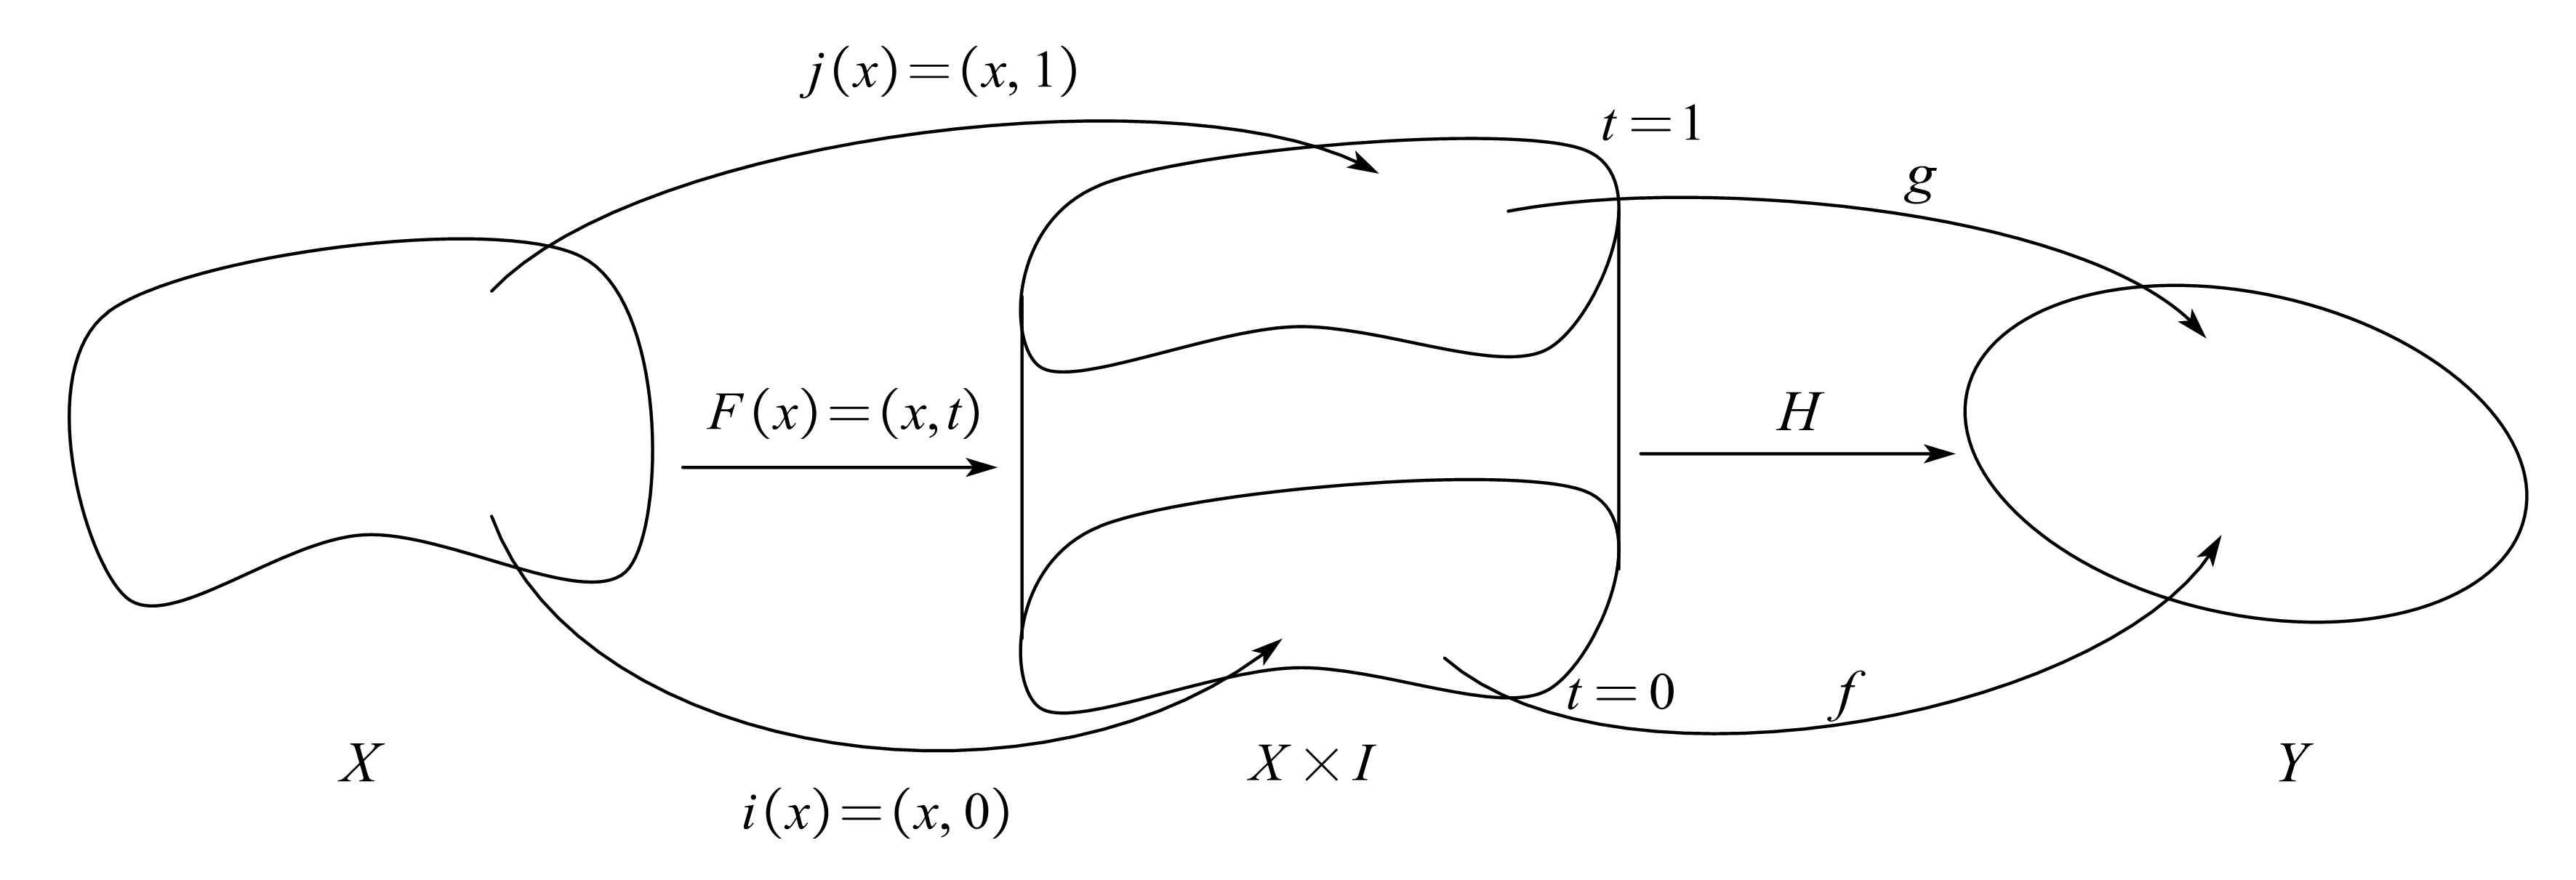
\includegraphics[width=0.75\linewidth]{figures/Sec10-2.png}
\end{figure}
若将 $ i,j $ 代数化得到 $ i_\sharp $, $ j_\sharp $, 只需要证明 $ i_\sharp $ 与 $ j_\sharp $ 链同伦, 那么
\[
	g_\sharp=H_\sharp j_\sharp,\qquad f_\sharp=H_\sharp i_\sharp.
\]
如果可以找到 $ D_X : S_p(X)\to S_{p+1}(X\times I) $ 使得 $ \partial D_X+D_X\partial=j_\sharp-i_\sharp $, 那么它复合上 $ H $ 诱导的链映射 $ H_\sharp : S_{p+1}(X\times I)\to S_p(Y) $ 就使得 $ D:=H_\sharp D_X : S_p(X)\to S_p(Y) $ 是连接 $ g_\sharp $ 和 $ f_\sharp $ 的链同伦. 这因
\[
	\partial D+D\partial=\partial H_\sharp D_X+H_\sharp D_X\partial=H_\sharp(\partial D_X+D_X\partial)=H_\sharp(j_\sharp-i_\sharp)=g_\sharp-f_\sharp.
\]

\begin{Lemma}\label{lem:同伦公理的引理}
	$ i_\sharp\simeq j_\sharp $.
\end{Lemma}
\begin{Proof}
	我们需要构造这样的 $ D_X : S_p(X)\to S_{p+1}(X\times I) $ 使得
	\[
		\partial D_X+D_X\partial=j_\sharp-i_\sharp,
	\]
	且图
	\begin{center}
		\begin{tikzcd}
			S_p(X) \arrow[r, "D_X"] \arrow[d, "f_\sharp"] & S_{p+1}(X\times I) \arrow[d, "(f\times\id_{I})_\sharp"] \\
			S_p(Y) \arrow[r, "D_Y"]                       & S_{p+1}(Y\times I)                                     
		\end{tikzcd}
	\end{center}
	交换.

	当 $ p=0 $ 时, 观察 $ D_X : S_0(X)\to S_1(X\times I) $, 取 $ T\in C(\Delta_0,X) $, 考虑 $ T(\Delta_0)=x_0 $
	\[
		D_X(T) : \Delta_1\to X,\qquad (t_0,0,\dots,)=(x_0,t),
	\]
	其中 $ 0\leqslant t\leqslant 1 $. 此时
	\[
		\partial D_X(T)=D_X(T)\circ\ell[\hat{\varepsilon}_0,\varepsilon_1]-D_X(T)\circ\ell[\varepsilon_0,\hat{\varepsilon}_1]=j_\sharp(T)-i_\sharp(T).
	\]
	这因
	\[
		D_X(T)\circ\ell[\hat{\varepsilon}_0,\varepsilon_1](\Delta_0)=D_X(T)(1,0,\dots,)=(x_0,1)=j_\sharp(T)(\Delta_0),
	\]
	类似地有 $ t=0 $ 的情况. 再验证 $ D_X $ 的函子性, 对任意 $ T : \Delta_0\in X $ 和任意 $ (t,0,\dots)\in\Delta_1 $, 有
	\[
		D_Yf_\sharp(T)(t,0,\dots)=D_X(f\circ T)(t,0,\dots)=(f(x_0),t)
	\]
	和
	\[
		(f\times\id_I)_\sharp D_X(T)(t,0,\dots)=(f\times\id_I)_\sharp(x_0,t)=(f(x_0),t)
	\]
	可知图交换.

	下面假设 $ <p $ 的情形都成立, 考虑 $ p $ 维链群上的 $ D_X $: 首先考虑特殊情形, 当 $ X=\Delta_p $ 时, 我们需要定义一个这样的 $ D_{\Delta_p} $, 如果它存在, 应当有
	\[
		\partial D_{\Delta_p}(\id_{\Delta_p})=\hat{\jmath}_\sharp(\id_{\Delta_p})-\hat{\imath}(\id_{\Delta_p})-D_{\Delta_p}(\partial\id_{\Delta_p}),
	\]
	而后三项都有定义(\textit{注意到 $ \partial\id_{\Delta_p}\in S_{p-1}(\Delta_p) $}), 又因 $ \Delta_p $ 零调, 于是 $ Z_p(\Delta_p)=B_p(\Delta_p) $. 因此只需 $ \partial D_{\Delta_p}(\id_{\Delta_p})=c_p\in Z_p(\Delta_p) $ 即可.

	\begin{figure}[htbp]
		\centering
		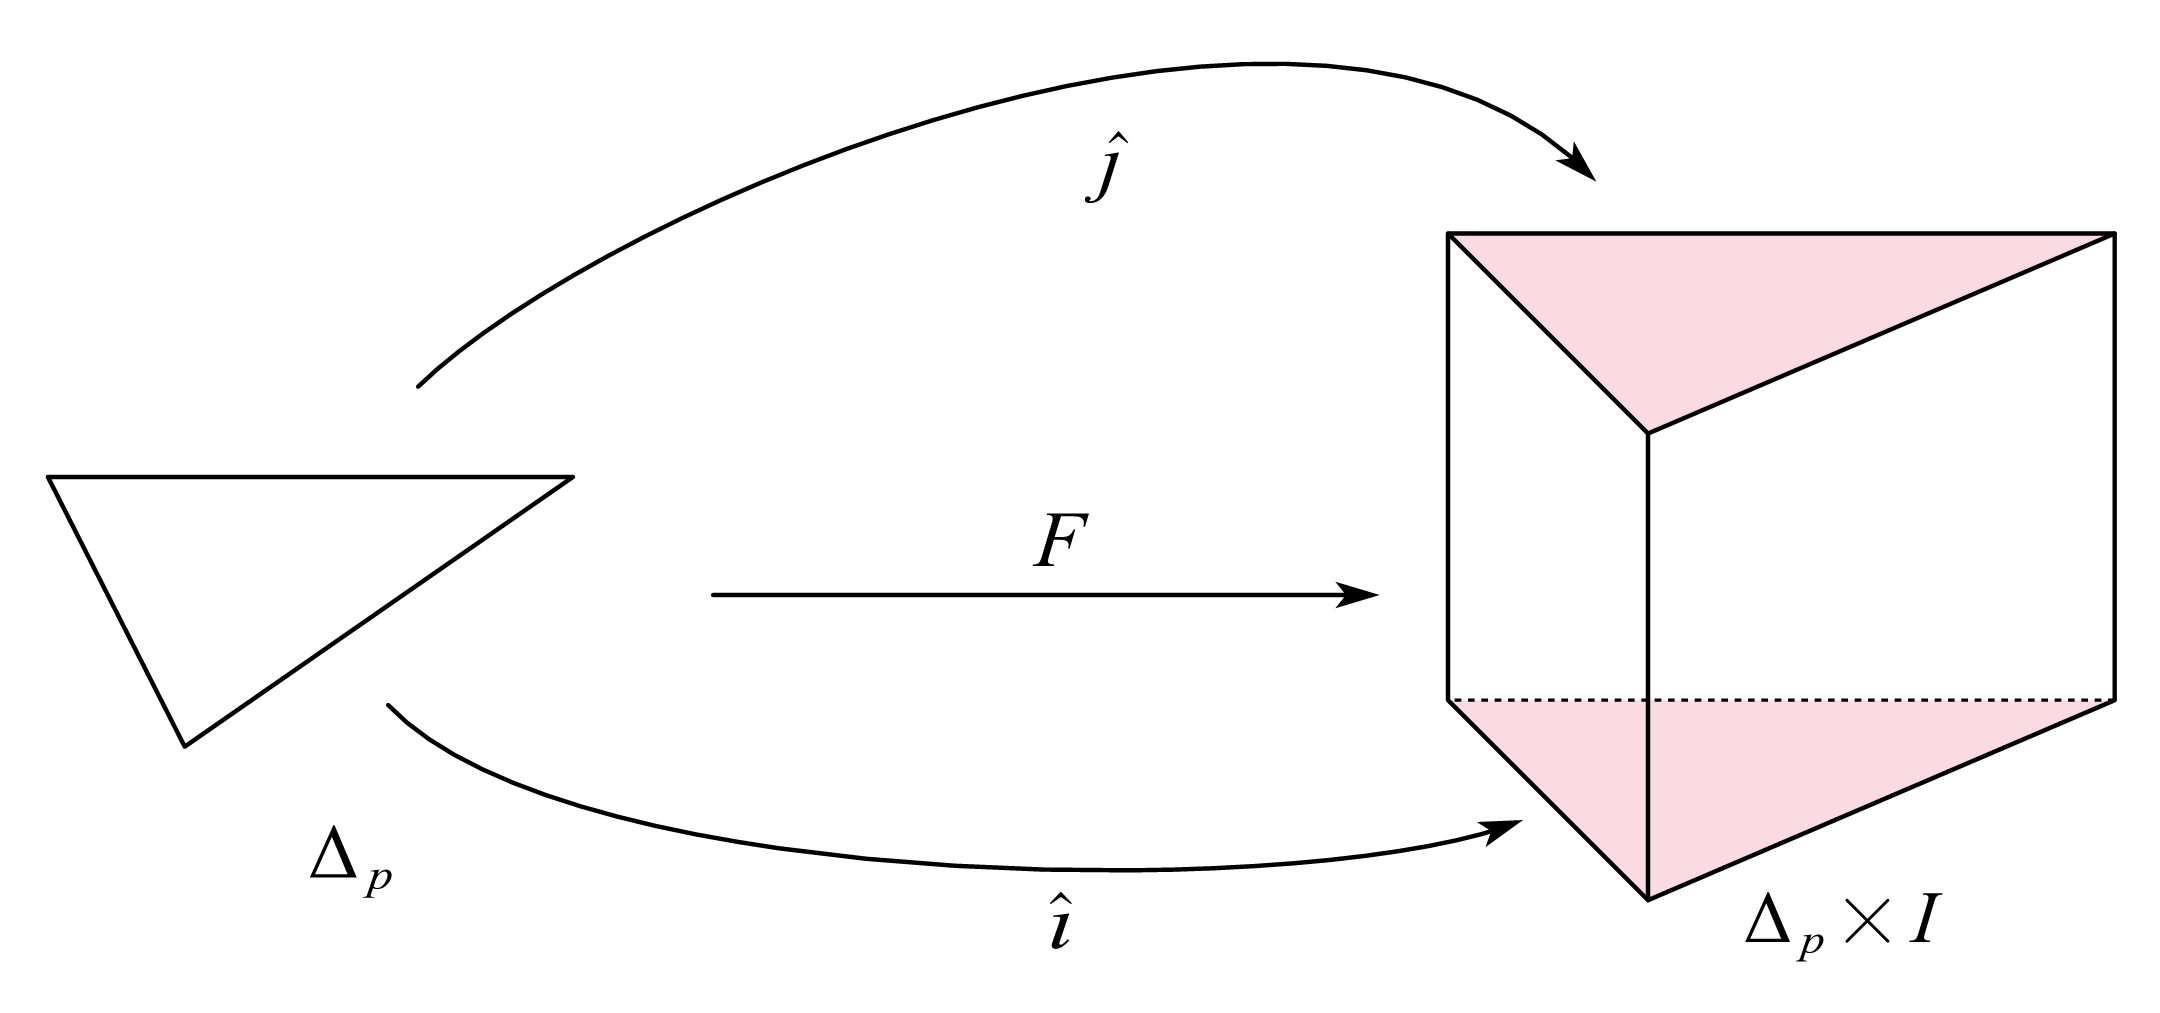
\includegraphics[width=0.4\linewidth]{figures/Sec10-3.png}
	\end{figure}
	直接计算验证即可:
	\[
		\begin{aligned}
			\partial c_p&=\partial(\hat{\jmath}_\sharp(\id_{\Delta_p})-\hat{\imath}_\sharp(\id_{\Delta_p})-D_{\Delta_p}(\partial\id_{\Delta_p}))\\
			&=\partial\hat{\jmath}(\id_{\Delta_p})-\partial\hat{\imath}(\id_{\Delta_p})-(\hat{\jmath}_\sharp(\partial\id_{\Delta_p})-\hat{\imath}_\sharp(\partial\id_{\Delta_p})-\partial D_{\Delta_p}(\partial\id_{\Delta_p}))\\
			&=0.
		\end{aligned}
	\]
	于是 $ c_p\in Z_p(\Delta_p)=B_p(\Delta_p) $, 则存在 $ d\in S_{p+1}(\Delta_p) $ 使得 $ \partial d=c_p $, 取 $ D_{\Delta_p}(\id_{\Delta_p})=d $ 即可.

	现在任取 $ X $ 是一个拓扑空间, 定义
	\[
		D_X : S_p(X)\to S_{p+1}(X\times I),\qquad T : \Delta_p\to X\mapsto D_X(T) :=(T\times\id_I)_\sharp D_{\Delta_p}(\id_{\Delta_p}).
	\]
	\begin{figure}[htbp]
		\centering
		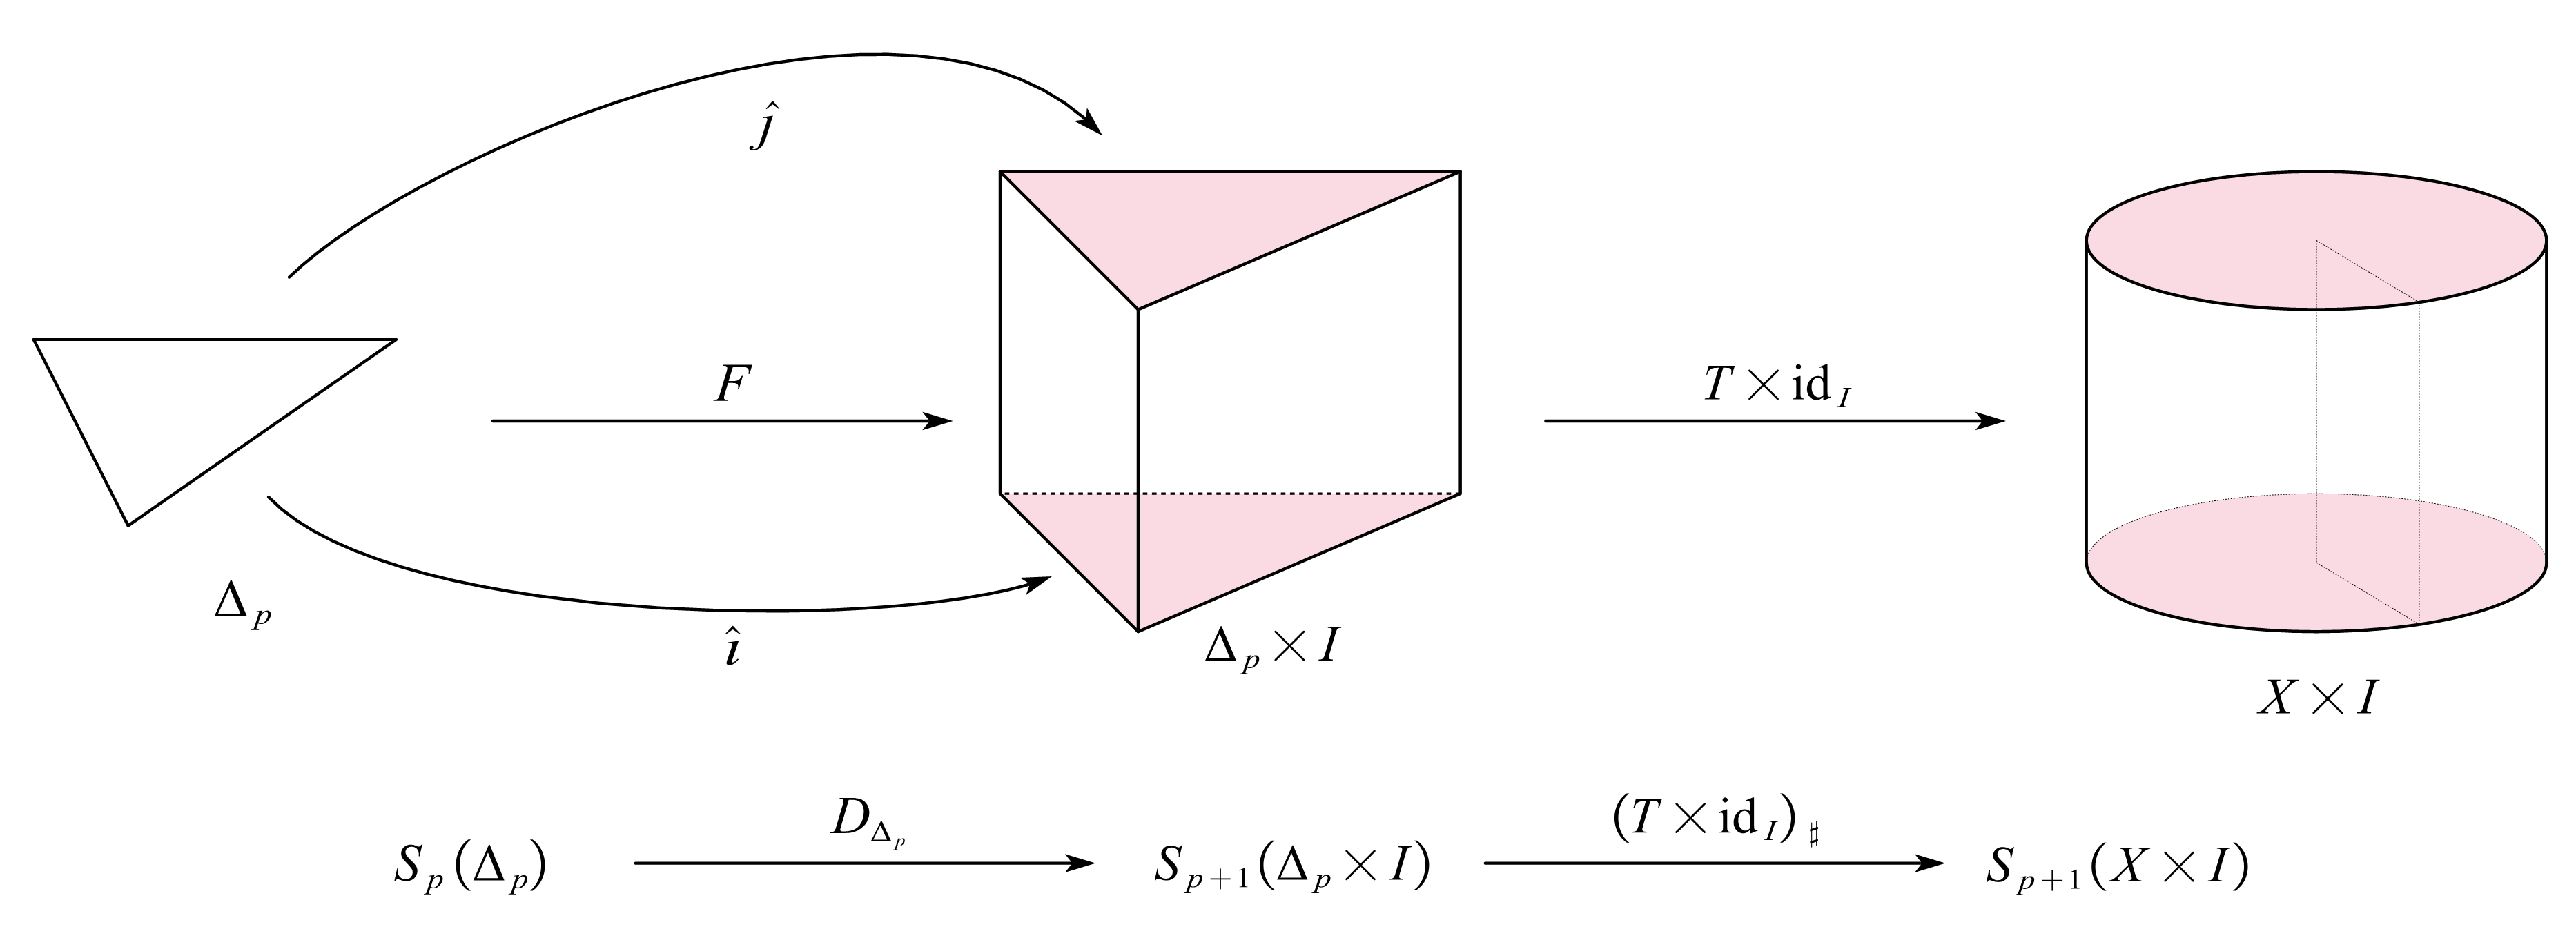
\includegraphics[width=0.75\linewidth]{figures/Sec10-4.png}
	\end{figure}

	下面只需验证 $ \partial D_X=D_X\partial=j_\sharp-i_\sharp $ 即可. 对任意 $ T\in S_p(X) $
	\[
		\begin{aligned}
			\partial D_X(T)&=\partial((T\times\id_I)_\sharp D_{\Delta_p}(\id_{\Delta_p}))\\
			&=(T\times\id_I)_\sharp\partial D_{\Delta_p}(\id_{\Delta_p})\\
			&=(T\times\id_I)_\sharp(\hat{\jmath}(\id_{\Delta_p})-\hat{\imath}(\id_{\Delta_p})-D_{\Delta_p}(\partial\id_{\Delta_p}))\\
			&=j_\sharp(T)-i_\sharp(T)-(T\times\id_{I})_\sharp D_{\Delta_p}(\partial\id_{\Delta_p})\\
			&=j_\sharp(T)-i_\sharp(T)-D_XT_\sharp(\partial\id_{\Delta-p})\\
			&=j_\sharp(T)-i_\sharp(T)-D_X\partial T_\sharp(\id_{\Delta_p})\\
			&=j_\sharp(T)-i_\sharp(T)-D_X\partial(T).
		\end{aligned}
	\]
	再验证 $ D_X $ 在 $ S_p $ 上的函子性. 对任意 $ T : \Delta_p\to X $ 和 $ f : X\to Y $, 有
	\[
		D_Yf_\sharp(T)=D_Y(f\circ T)=((f\circ T)\times\id_I)_\sharp D_{\Delta_p}(\id_{\Delta_p})
	\]
	和
	\[
		(f\times\id_I)_\sharp D_X(T)=(f\times\id_I)_\sharp\circ(T\times\id_I)_\sharp D_{\Delta_p}(\id_{\Delta_p})=((f\circ T)\times\id_I)_\sharp D_{\Delta_p}(\id_{\Delta_p}),
	\]
	于是在 $ S_p $ 上图表交换.

	由归纳法可知命题成立.\qed
\end{Proof}

\begin{Theorem}
	若 $ f\simeq g $, 则 $ f_*=g_* $.
\end{Theorem}

这一定理实际上就是 (5), 其证明由引理~\ref{lem:同伦公理的引理}~和它上面的讨论得到.

对奇异链, 一般来说 $ \CS(X_1)\otimes\CS(X_2)\to\CS(X) $ 并不是满的, 因为可能出现下图这样的状况:
\begin{figure}[htbp]
	\centering
	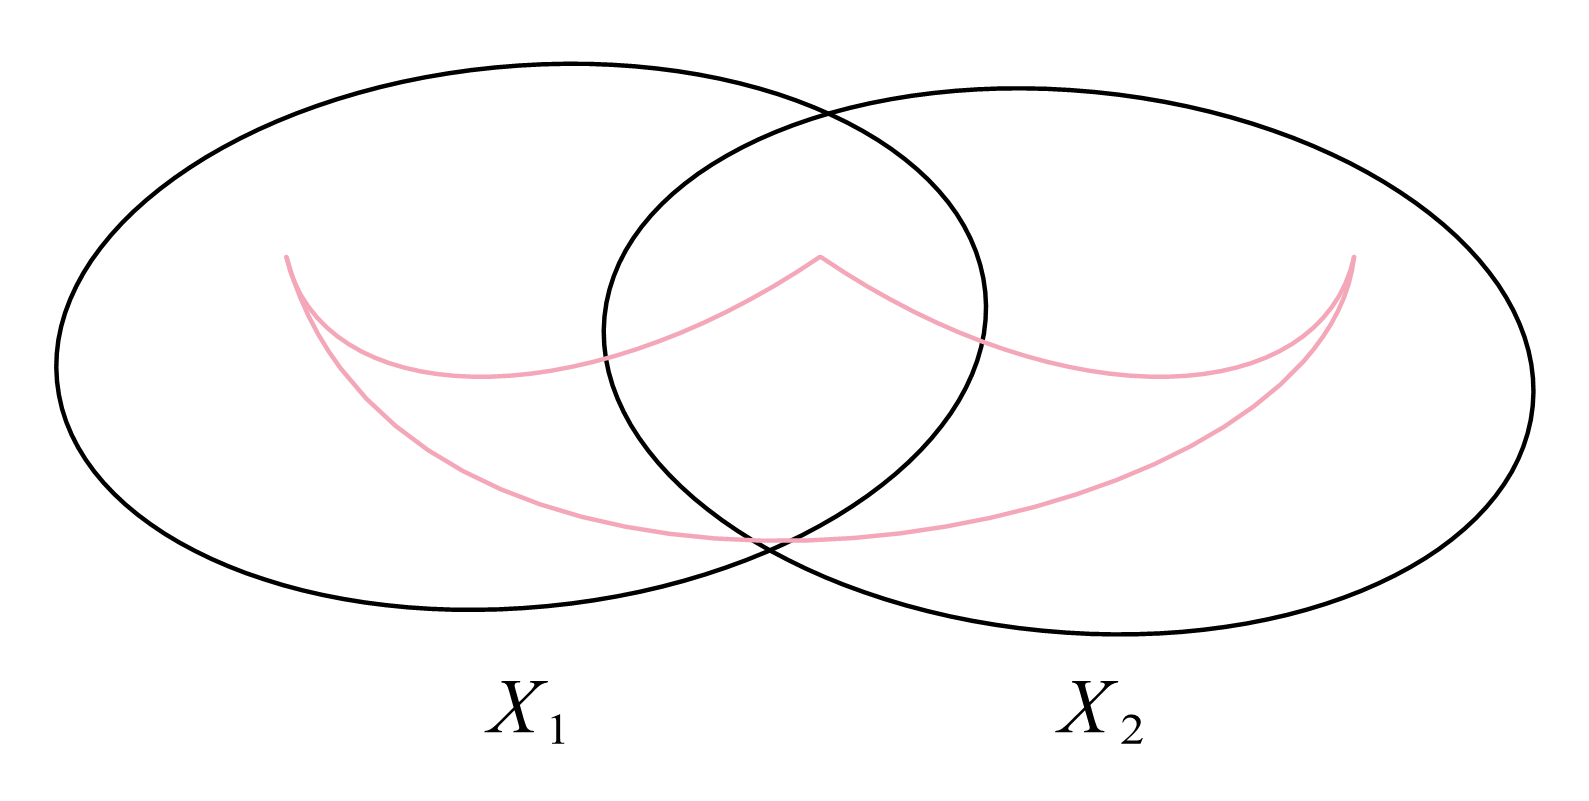
\includegraphics[width=0.3\linewidth]{figures/Sec11-1.png}
\end{figure}\\
但对
\begin{center}
	\begin{tikzcd}
		& X_1 \arrow[rd, "k", hook] &   \\
		  X_1\cap X_2 \arrow[ru, "i", hook] \arrow[rd, "j", hook] &                           & X \\
		& X_2 \arrow[ru, "l", hook] &  
	\end{tikzcd}
\end{center}
它仍然可以诱导短正合列
\begin{center}
	\begin{tikzcd}
		0 \arrow[r] & \CS(X_1\cap X_2) \arrow[r] & \CS(X_1)\oplus\CS(X_2) \arrow[r] & \CS(X_1)+\CS(X_2) \arrow[r] & 0 \\
					& c \arrow[r, maps to]       & {(i_\sharp(c),-j_\sharp(c))}     &                             &   \\
					&                            & {(c_1,c_2)} \arrow[r, maps to]   & c_1+c_2                     &  
	\end{tikzcd}
\end{center}
由 zig--zag 引理可知它诱导长正合列
\begin{center}
	\begin{tikzcd}
		{} \arrow[r] & H_p(X_1\cap X_2) \arrow[r] & H_p(X_1)\oplus H_p(X_2) \arrow[r] & H_p(\CS(X_1)+\CS(X_2)) \arrow[r] & H_{p-1}(X_1\cap X_2) \arrow[r] & {}
	\end{tikzcd}
\end{center}
我们当然希望 $ H_p(\CS(X_1)+\CS(X_2))\cong H_p(X) $, 这样上面的序列就是 Mayer--Vietoris 序列.

\begin{Definition}[切除对]
	设 $ X=X_1\cup X_2 $, 若
	\[
		\CS(X_1)+\CS(X_2)\hookrightarrow\CS(X),
	\]
	诱导同调群的同构, 也即 $ H_p(\CS(X_1)+\CS(X_2))\cong H_p(X) $, 则称 $ (X_1,X_2) $ 是 $ X $ 的一个\emph{切除对}.
\end{Definition}

\begin{Theorem}
	若 $ (X_1,X_2) $ 是 $ X $ 的切除对, 则存在长正合列
	\begin{center}
		\begin{tikzcd}
			{} \arrow[r] & H_p(X_1\cap X_2) \arrow[r] & H_p(X_1)\oplus H_p(X_2) \arrow[r] & H_p(X) \arrow[r] & H_{p-1}(X_1\cap X_2) \arrow[r] & {}
		\end{tikzcd}
	\end{center}
	此即切除对 $ (X_1,X_2) $ 的 \emph{Mayer--Vietoris 序列}.
\end{Theorem}

但直接从定义出发构造切除对太过困难, 下面提供一个简单的构造切除对的方法.

\begin{Lemma}
	$ (X_1,X_2) $ 是 $ X $ 的切除对当且仅当 $ (X_1,X_1\cap X_2)\hookrightarrow(X,X_2) $ 诱导同调群的同构.(\textit{此即 Munkres 书中习题26-3}).
\end{Lemma}
\begin{Proof}
	我们有
	\begin{center}
		\begin{tikzcd}
			0 \arrow[r] & \CS(X_2) \arrow[r, hook]                                & \CS(X) \arrow[r, two heads]                            & {\CS(X,X_2)} \arrow[r]                           & 0 \\
			0 \arrow[r] & \CS(X_2) \arrow[r, hook] \arrow[u, Rightarrow, no head] & \CS(X_1)+\CS(X_2) \arrow[r, two heads] \arrow[u, hook] & {\CS(X_1,X_1\cap X_2)} \arrow[r] \arrow[u, hook] & 0
			\end{tikzcd}
	\end{center}
	其中上下两行都是正合的. 下方的序列正合因取 $ \pi : \CS(X_1)+\CS(X_2)\to\CS(X_1,X_1\cap X_2) $ 使得 $ \ker\pi=\CS(X_2) $. 它们会诱导长正合列
	\begin{center}
		\begin{tikzcd}
			{} \arrow[r] & {H_{p+1}(X,X_2)} \arrow[r]                     & H_p(X_2) \arrow[r]                                & H_p(X) \arrow[r]                           & {H_p(X,X_2)} \arrow[r]                       & H_{p-1}(X_2) \arrow[r]                                & {} \\
			{} \arrow[r] & {H_{p+1}(X_1,X_0)} \arrow[r] \arrow[u] & H_p(X_2) \arrow[r] \arrow[u, Rightarrow, no head] & H_p(\CS(X_1)+\CS(X_2)) \arrow[r] \arrow[u] & {H_{p}(X_1,X_0)} \arrow[r] \arrow[u] & H_{p-1}(X_2) \arrow[r] \arrow[u, Rightarrow, no head] & {}
		\end{tikzcd}
	\end{center}
	其中 $ X_0=X_1\cap X_2 $. 由五引理得证.\qed
\end{Proof}

\begin{Proposition}
	若 $ \set{\mathrm{Int}\,X_1,\mathrm{Int}\,X_2} $ 是 $ X $ 的开覆盖, 则 $ (X_1,X_2) $ 是 $ X $ 的切除对.
\end{Proposition}
\begin{Proof}
	不失一般性, 不妨 $ X_1 $ 和 $ X_2 $ 都是开集, 那么取 $ U=X_2\sm(X_1\cap X_2) $, 则
	\[
		\bar{U}=\baro{X_2\sm(X_1\cap X_2)}\subset X_2=\mathrm{Int}\,X_2,
	\]
	由切除公理, 有
	\[
		H_p(X,X_2)\cong H_p(X\sm U,X_2\sm U)=H_p(X_1,X_1\cap X_2),
	\]
	得证.\qed
\end{Proof}

\begin{Example}[球面的一点并]
	设 $ X=\S^m\vee\S^n $, $ m,n>0 $, 取 $ X_1=\S^m $, $ X_2=\S^n $, 则 $ (X_1,X_2) $ 是 $ X $ 的切除对. 我们有 Mayer--Vietoris 序列
	\[
		\to H_p(\mathrm{pt})\rightarrow H_p(X_1)\oplus H_p(X_2)\rightarrow H_p(X)\rightarrow H_{p-1}(\mathrm{pt})\to
	\]
	因 $ X $ 道路连通, 故 $ H_0(X)\cong\Z $. 当 $ p>0 $ 时, 由 Mayer--Vietoris 序列可知
	\[
		H_p(X)\cong\begin{cases}
			\Z\oplus\Z &,p=m=n \\ 0 &,p\ne m
		\end{cases}\qquad H_p(X)\cong\begin{cases}
			\Z &,p=m \\ \Z &,p=n \\ 0 &,p\ne m,\ p\ne n.
		\end{cases}
	\]
\end{Example}

\begin{Example}[锥和悬挂(双锥)]
	考虑拓扑空间 $ X $, 它的\emph{锥}和\emph{悬挂}(或\emph{双锥})可以分别看作以下的商空间:
	\[
		w*X:=(X\times I)/(X\times\set{1})
	\]
	和
	\[
		S(X):=(X\times[-1,1])/(X\times\set{1}\cup X\times\set{-1}).
	\]
	将悬挂看作是对空间的一元运算, 那么映射 $ S : X\mapsto S(X) $ 可以对自身复合, 归纳地定义 $ S^{n+1}(X):=S(S^n(X)) $.
	\begin{figure}[htbp]
		\centering
		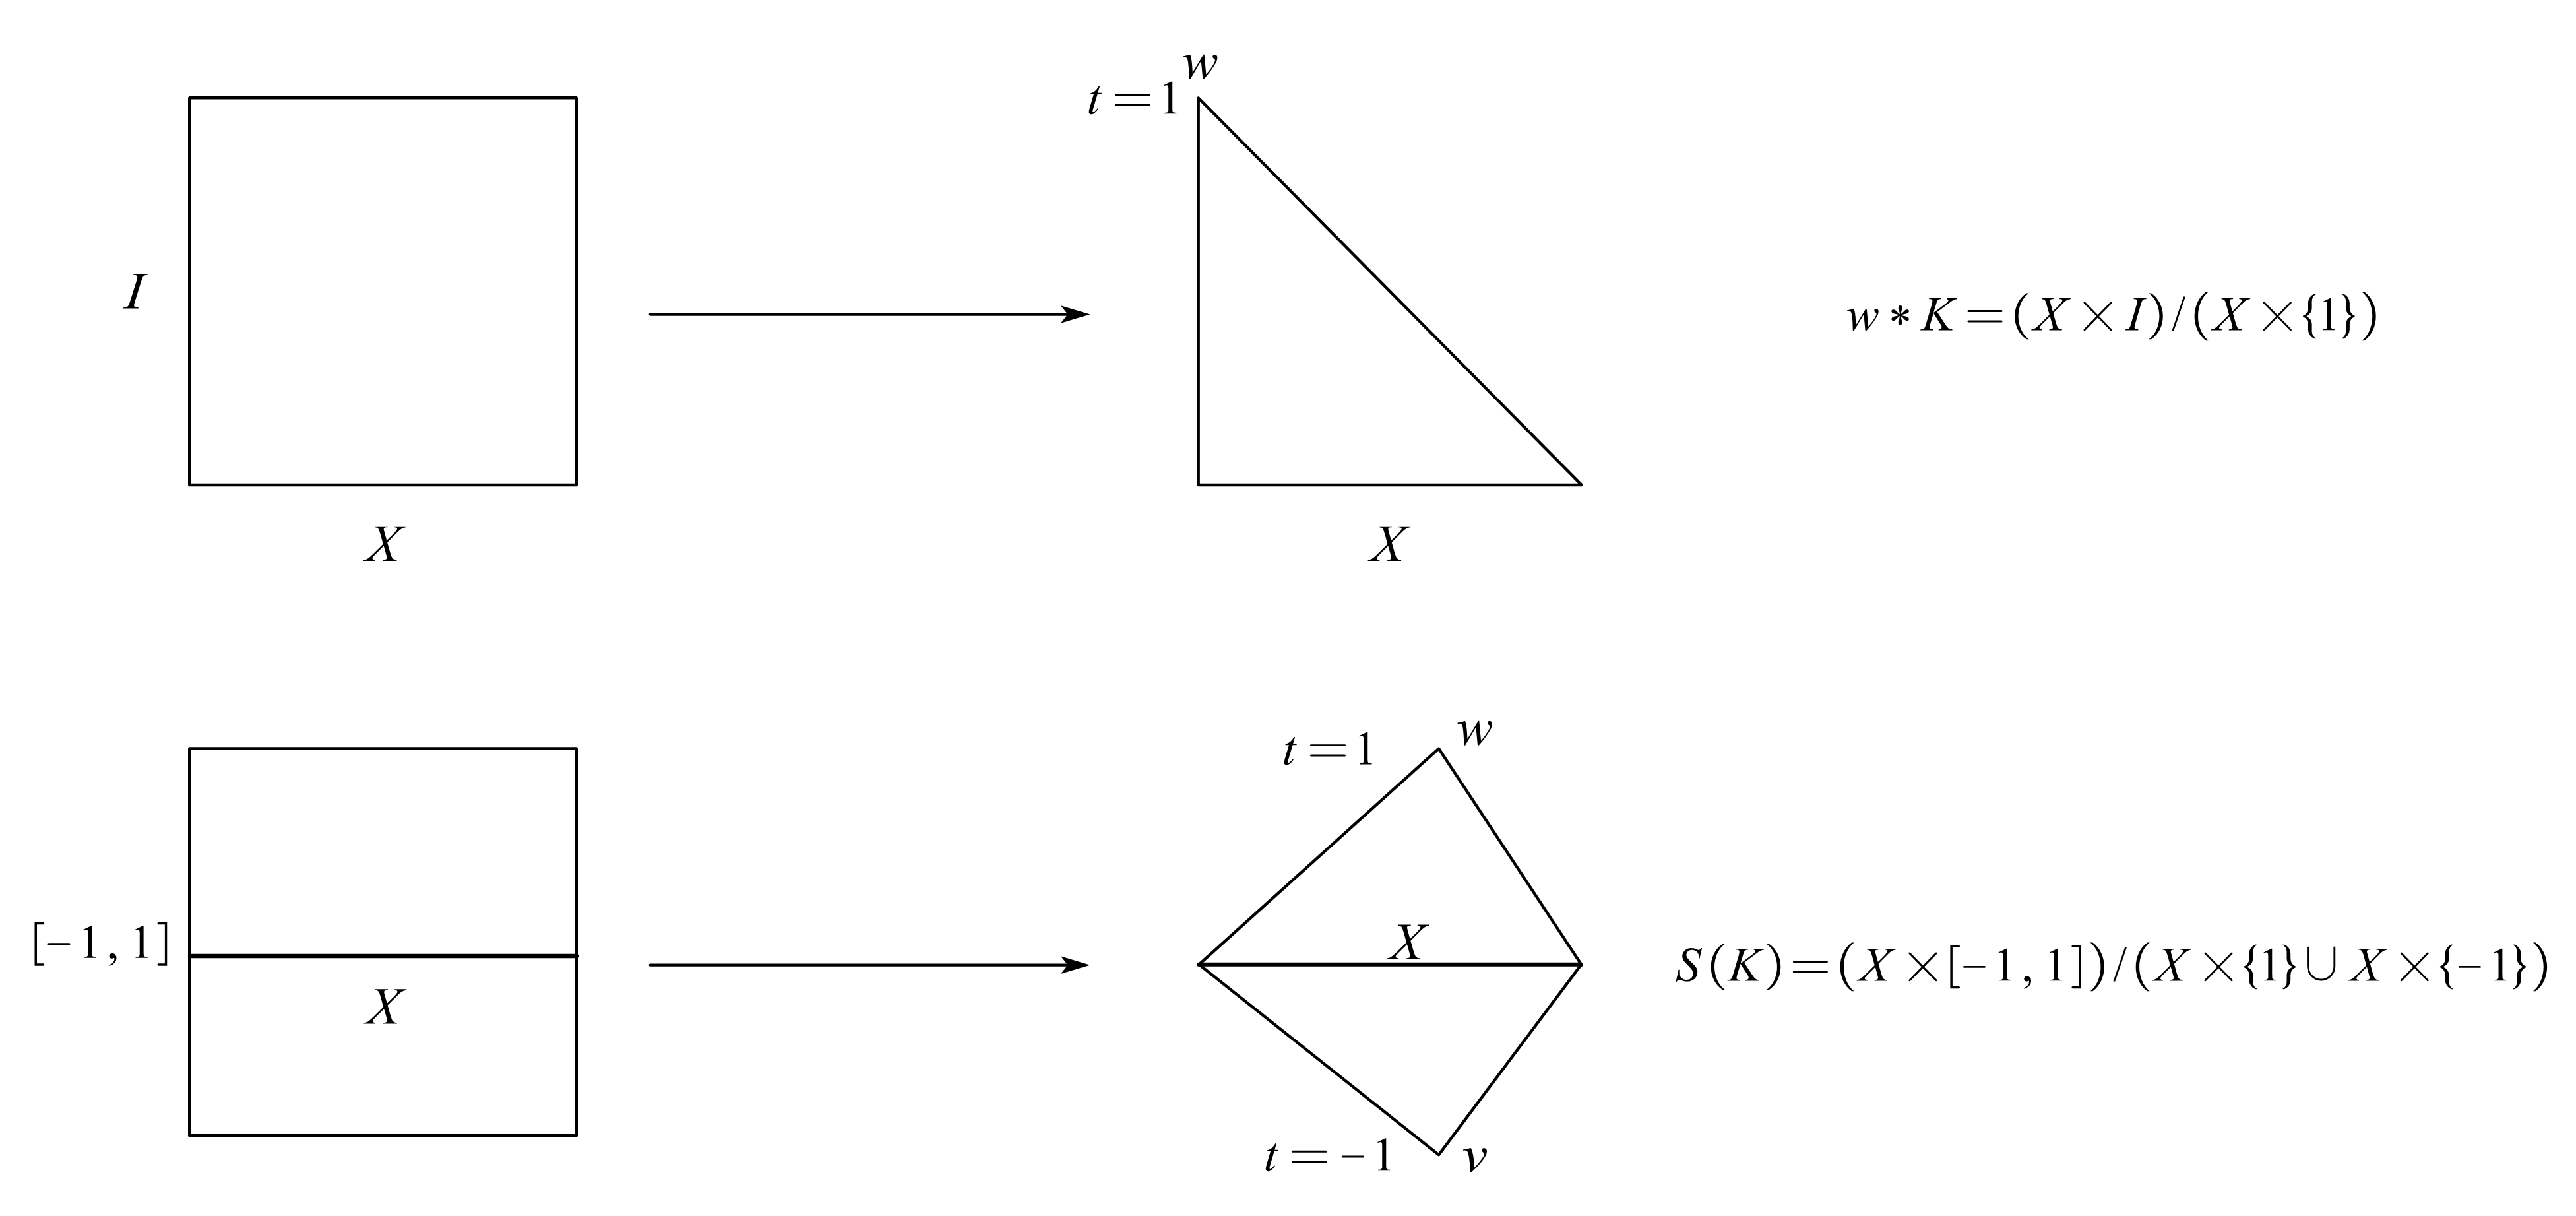
\includegraphics[width=0.85\linewidth]{figures/Sec11-2.png}
	\end{figure}
\end{Example}

锥总是零调的, 于是讨论锥的同调群没什么价值. 但双锥一般情况下并不是可缩的, 于是我们还是需要探讨一下 $ S(X) $ 和 $ X $ 的同调群之间的关系.

\begin{Theorem}
	$ H_p(S(X))\cong\tilde{H}_{p-1}(X) $.
\end{Theorem}
\begin{Proof}
	设 $ S(X) $ 的两个悬挂点为 $ v,w $, 记
	\[
		X_1=S(X)\sm\set{w},\qquad X_2=S(X)\sm\set{v},
	\]
	则 $ X_1,X_2 $ 是开集, 且 $ (X_1,X_2) $ 是 $ X $ 的切除对. 考虑投影 $ \pi $, 有
	\[
		\pi(X\times(-1,1])=X_1,\qquad\pi(X\times[-1,1))=X_2.
	\]

	考虑切除对 $ (X_1,X_2) $ 的 Mayer--Vietoris 序列,
	\[
		\to H_p(X_1)\oplus H_p(X_2)\rightarrow H_p(S(X))\rightarrow H_{p-1}(X_1\cap X_2)\rightarrow H_{p-1}(X_1)\oplus H_{p-1}(X_2)\to
	\]
	而 $ X_1 $, $ X_2 $ 都可缩, 于是
	\[
		\tilde{H}_p(X_1)=\tilde{H}_p(X_2)=0.
	\]
	对 $ X_1\cap X_2 $, 注意到投影 $ \pi $ 限制到 $ X\times(-1,1) $ 上是一个双射, 且 $ X\times\set{0} $ 是一个形变收缩核, 那么 $ X_1\cap X_2\simeq X $. 于是命题得证.\qed
\end{Proof}

\subsection{应用: 拓扑流形和局部同调群}

下面总假设 $ X $ 是一个 Hausdorff 空间, $ x\in X $, $ A $ 是 $ X $ 的邻域, $ U=X\sm A $. 那么
\[
	\bar{U}=\baro{X\sm A}\subset X\sm x=\mathrm{Int}\,(X\sm x),
\]
由切除公理可知
\[
	H_p(X,X\sm x)\cong H_p(A,A\sm x),
\]
这称作 $ x $ 处的\emph{局部同调}.

\begin{Example}
	对 $ X=\R^n $, 有
	\[
		H_p(\R^n,\R^n\sm\set{0})\cong H_p(\B^n,\B^n\sm\set{0})\cong H_p(\B^n,\S^{n-1})=\begin{cases}
			\Z &,p=n \\ 0 &,p\ne n.
		\end{cases}
	\]
	由此可导出对任何 $ m\ne n $, 都有 $ \R^m $ 和 $ \R^n $ 不同胚. 但在点集拓扑中, 要处理这样的问题是十分困难的.
\end{Example}

\begin{Definition}[拓扑流形]
	称 $ M $ 是一个\emph{拓扑流形}, 若 $ M $ 是 Hausdorff 的, 且对任意 $ x\in M $, 存在 $ U\in\CN(x) $ 使得存在同胚 $ \varphi : U\to\R^m $. 若在局部 $ M\cong\R^m $, 则称 $ M $ 是\emph{无边流形}, 若在局部 $ M\cong\H^m $, 则称 $ M $ 是\emph{带边流形}.
\end{Definition}

因此, 局部同调群可以用来确定一个流形的维数. 对无边流形 $ M $, 有
\[
	H_p(M,M\sm x)\cong H_p(\R^m,\R^m\sm \set{0})\cong\begin{cases}
		\Z &,p=m \\ 0 &,p\ne m.
	\end{cases}
\]
对带边流形 $ M $, 若 $ x\in\mathrm{Int}\,M $, 其局部同调与无边流形类似, 只是此时只有 $ p=m-1 $ 时 $ H_p(M,M\sm x)\cong\Z $; 若 $ x\in\mathrm{Bd}\,M $, 有
\[
	H_p(M,M\sm x)\cong H_p(\H^m,\H^m\sm\set{0})\cong H_p(\B^m_+,\B^m_+\sm\set{0})=0.
\]

一些有关拓扑流形的同调群的结论列举如下:

\begin{Theorem}
	设 $ M $ 是可三角剖分的带边流形, 若存在复形 $ K $ 使得 $ h : \abs{K}\to M $ 是一个同构, 则 $ h^{-1}(\mathrm{Bd}\,M) $ 是 $ K $ 的子复形的几何实现.
\end{Theorem}

\begin{Theorem}
	设 $ K $ 是 $ M $ 的一个三角剖分, $ v\in K^{(0)} $, 那么对任意 $ p\in\Z $ 成立
	\[
		H_p(M,M\sm h(v))\cong H_p(\baro{\mathrm{St}}\,v,\mathrm{Link}\,v).
	\]
\end{Theorem}